\documentclass[a4j,10pt,dvips,onecolumn,oneside,final]{jarticle}%{amsart}
\usepackage{wrapfig}
\usepackage{url}
\usepackage{graphicx}
\usepackage{fancyvrb}

% fancyvrb setting %
\fvset{
    tabsize=4,
    baselinestretch=0.8,
    numbers=none,
    frame=single,
    fontsize=\small,
%%     % framesep=5pt,
%%     % numbersep=5pt,
%%     % comment
}

\newcommand {\daqmwcurrent} {
	{\bf DAQ-Middleware 1.0.0}
}

\newcommand {\rtmcurrent} {
	{\bf OpenRTM-aist-1.0.0}
}

\setlength{\oddsidemargin}{0cm}
\setlength{\evensidemargin}{0cm}
\setlength{\textwidth}{16cm}
\setlength{\topmargin}{0cm}
\setlength{\textheight}{22cm}

\begin{document}

\title{ \daqmwcurrent 技術解説書\\
%  第1版(June 2009)
%  第2版(Oct. 2009)
%  第3版(Jun  2010)
}
\author{仲吉一男}
\date{
\vspace{0.1cm}
  KEK素核研\\
\vspace{0.4cm}
%  \\July 2009\\
%  Oct. 2009 (revised)
  2010年 8月 
%\vspace{0.5cm}
%{\small 高エネルギー加速器研究機構}\\ 
%\vspace{0.1cm} 
%{\small 素粒子原子核研究所}
}
\maketitle
%\thispagestyle{empty}
\begin{abstract}
この文書はユーザーがDAQコンポーネントを開発する際に必要となる
 \daqmwcurrent の仕様について技術的な解説をするために書かれました。
第\ref{arch}節でDAQミドルウェアのアーキテクチャの概要を説明し、
第\ref{daqcomp}節でDAQコンポーネントの仕様について説明します。
第\ref{daqop}節でDAQオペレータの仕様を説明します。

\end{abstract}
{\rm }
%\pagenumbering{roman}
\tableofcontents
%\cleardoublepage
%\pagenumbering{arabic}
%\setcounter{page}{1}
\newpage

\begin{wrapfigure}{r}{70mm}
  \begin{center}
   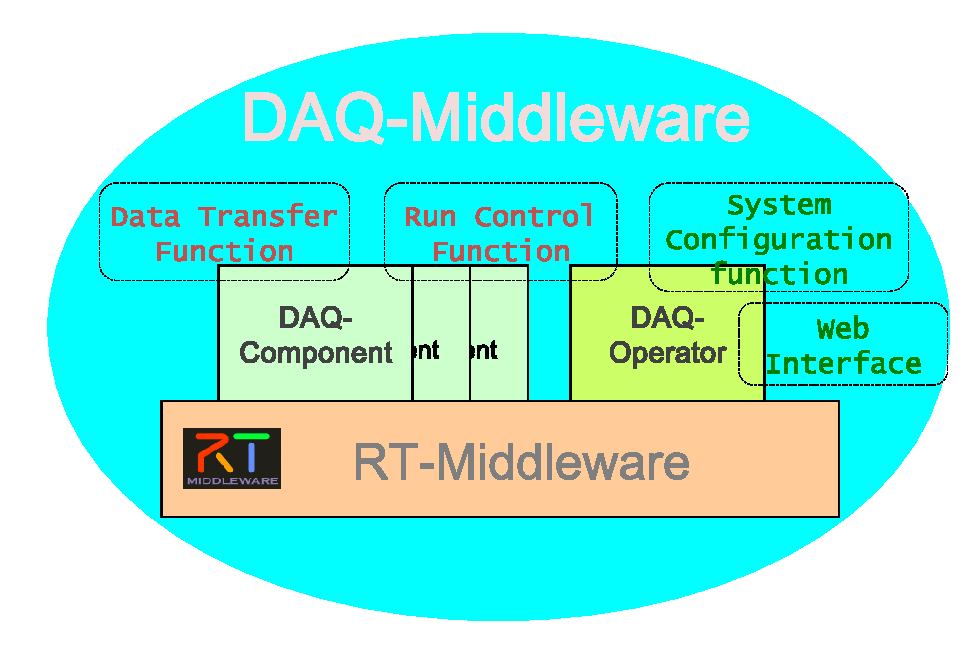
\includegraphics[width=70mm]{daqmw-rtmw.eps}
  \end{center}
  \vspace{-7mm}
  \caption{\footnotesize DAQミドルウェアとRTミドルウェアの関係}
  \label{daqmw.fig}
\end{wrapfigure}

\section{はじめに}\label{intro}
この文書はユーザーがDAQコンポーネントを開発する際に必要となる
\daqmwcurrent の仕様について技術的な解説をするために書かれました。
第\ref{arch}節でDAQミドルウェアのアーキテクチャの概要、第\ref{daqcomp}節で
DAQコンポーネントの仕様について説明します。第\ref{daqop}節でDAQオペレータの仕様を説明します。

DAQ(Data AQuisition)ミドルウエアは、ネットワーク分散環境でデータ収集用ソフトウェアを容易
に構築するためのソフトウェア・フレームワークです。ユーザは、DAQコンポーネントと呼ばれる
ソフトウェア・コンポーネントを組み合わせてDAQシステムを構築します。

DAQミドルウエアの実装は、RT(Robot Technology) ミドルウェア\cite{RTM}技術をベースにしています。
RTミドルウエアは、独立行政法人産業技術総合研究所(AIST)により研究・開発が行われています。
RTミドルウェアは様々なロボット要素(RTコンポーネント)を通信ネットワークを介して自由に
組み合わせることで、ロボットシステムの構築を可能にするネットワーク分散コンポーネント化
技術による共通プラットフォームです。
RTミドルウエアの基本ソフトウェアであるRTコンポーネントは、ソフトウエアの国際標準化団体
OMG(Object Management Group)で標準仕様が採択され国際標準規格 
"Robotic Technology Component Specification"\cite{RTM-OMG}となりました。
我々は、RTコンポーネントをベースとするロボット・ネットワーク分散モデルは、データ収集に
も適用可能であると考え2006年からAISTと共同研究を開始し、その実現可能性の検討を行って
きました\cite{CHEP06}。%%\cite{CHEP06,RT07}。
その結果、RTコンポーネントに一部拡張を行うことでデータ収集においても適用可能である
という結論に至りました。
RTミドルウェアは、OMGによる国際標準化後も開発が続いています。この文書では、RTミドルウェア
の産総研による実装である
\rtmcurrent (\verb|C++|版)
を基に開発された
\daqmwcurrent(以降DAQミドルウェア)
について説明します。

図 \ref{daqmw.fig}にRTミドルウェアとDAQミドルウェアの関係を示した概念図を
示します。DAQコンポーネントは前述のRTコンポーネントを拡張して設計されています。すなわち、
(1)データ収集に必要なコマンドによる状態遷移の実装、(2)RTコンポーネントのサービスポートを
利用したコマンド/ステータス送受信機能の実装です。
またRTコンポーネントから受け継いだデータ入出力ポートによりDAQコンポーネント間でデータ転送
を行います。
DAQオペレータは、DAQコンポーネントを制御するためのコントローラです。
ユーザから「スタート」や「ストップ」というコマンドを受け、それをDAQコンポーネントへ
送信します。
また、XML文書によるDAQシステムのコンフィグレーション機能、XML/HTTPプロトコルを使用した
システム・インターフェイス機能を持っています。

DAQミドルウェアの概要のみを知りたい方は、「DAQミドルウェア概要\cite{OVERVIEW}」をご覧ください。

\section{DAQミドルウェアのアーキテクチャ}\label{arch}
DAQミドルウェアのアーキテクチャについて下記の項目の説明をします。
\begin{itemize}
\item ソフトウェア・コンポーネント・モデル(\ref{compmodel})
\item 状態遷移モデル(\ref{statemodel})
\item ランコントロール・モデル(\ref{runctrl})
\item データ転送機能(\ref{data-tarans})
\item コマンド・ステータス通信機能(\ref{status})
\item システム・コンフィグレーション機能(\ref{config})
\item システム・インターフェイス機能(\ref{sysint})
\item 装置パラメータ設定機能(\ref{cond})
\item リモートブート機能(\ref{remoteboot})
\end{itemize}

\subsection{ソフトウェア・コンポーネント・モデル}\label{compmodel}
DAQコンポーネントは、DAQミドルウェアにおけるソフトウェアの基本単位です。
色々な機能のDAQコンポーネントを組み合わせることで、柔軟なDAQシステムを構築できます。
ソフトウェア・コンポーネント指向のフレームワークを用いることで、次のことが期待できます。
\begin{itemize}
\item 柔軟なDAQシステムの構築の実現
%%\item マルチコアCPU 上において複数のコンポーネントの効率動作実現
\item ソフトウェア開発効率の向上
\item ソフトウェア再利用性の向上
\item ソフトウェアメンテナンス容易性の向上
\end{itemize}

前述のようにRTミドルウェアにおけるソフトウェアの基本単位がRTコンポーネントです。
ロボットシステムを構築するためには、センサ等のデバイスを組み合わせて実現しますが、
その機能要素をソフトウェア・コンポーネントで実現し、複数組み合わせることにより
システムを構築することが可能です。RTコンポーネントのアーキテクチャを
図\ref{RT-component.fig}に示します。
DAQコンポーネントを説明する上で重要なRTコンポーネントの要素は以下のものです。
\begin{itemize}
\item 状態(ステート)
\item 任意の数のデータ入力ポート(InPort)
\item 任意の数のデータ出力ポート(OutPort)
\item ユーザが定義可能なサービスポート
\end{itemize}
その他の機能や要素については、RTミドルウェアのページ等\cite{RTM, RTM-book}を参照して
ください。RTコンポーネントの状態遷移モデルについては後述します。
InPort,  OutPort はRTコンポーネント間を流れるデータストリームの入出力ポートです。
Publisher/Subscriberモデルに基づきコンポーネント間のデータの送受信を抽象化しています。
DAQコンポーネントでも同様に、InPort,  OutPortをデータの送受信に使用しています。
サービスポートはユーザが任意のサービスインターフェースを定義できるポートです。
「サービスプロバイダ」はサービスを提供するためのインターフェースで「サービス
コンシューマ」はサービスを利用するためのインターフェースです。
DAQコンポーネントでは、このサービスポートを利用してDAQオペレータとDAQコンポーネント
間のコマンド/ステータスの送受信を実装しています。
\begin{figure}[htbp]
 \begin{center}
  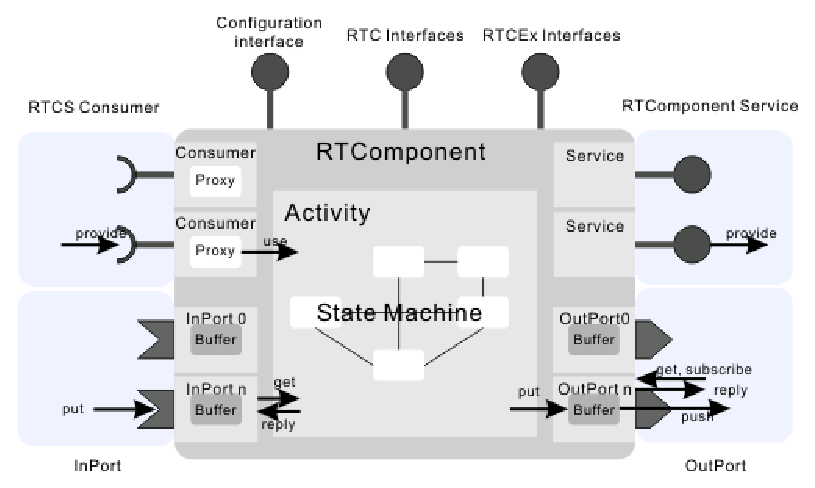
\includegraphics[width=100mm]{RT-component.eps}
  \caption{RTコンポーネントのアーキテクチャ}
  \label{RT-component.fig}
 \end{center}
\end{figure}

\subsection{状態遷移モデル}\label{statemodel}
図\ref{rtc-state.fig}にRTコンポーネントのステートチャートを示します。RTコンポーネントは
"Active", "Inactive", "Error"という状態間を遷移します。図\ref{daq-state.fig}にDAQ
コンポーネントのステートチャートを示します。我々の考える一般的なDAQシステムの4つの状態、
すなわち、"Loaded","Configured","Running","Paused"をRTコンポーネントの状態へ素直に
マッピングすることはできないため、RTコンポーネントの"Active"状態のサブ・ステートとして
実装しました。これにより、RTコンポーネントの状態遷移モデルを変更せずに DAQに必要な
状態を拡張することができました。
図\ref{command-state.fig}にDAQコンポーネントのコマンドによる状態遷移モデルを示します。
\begin{itemize}
\item DAQコンポーネントが起動すると"Loaded"状態となります。
\item "Loaded"状態では"Configure"コマンドによりDAQコンポーネントのパラメータの設定等を
行い"Configured"状態になります。
\item "Configured"状態では"Start"コマンドにより "Running"状態へ遷移します。
\item "Running"状態では "Pause"コマンドにより "Paused"状態へ遷移します。
\item "Paused"状態では "Resume"コマンドで"Running"状態へ遷移します。
\end{itemize}

\begin{figure}[htbp]
 \begin{minipage}{0.48\hsize}
  \begin{center}
   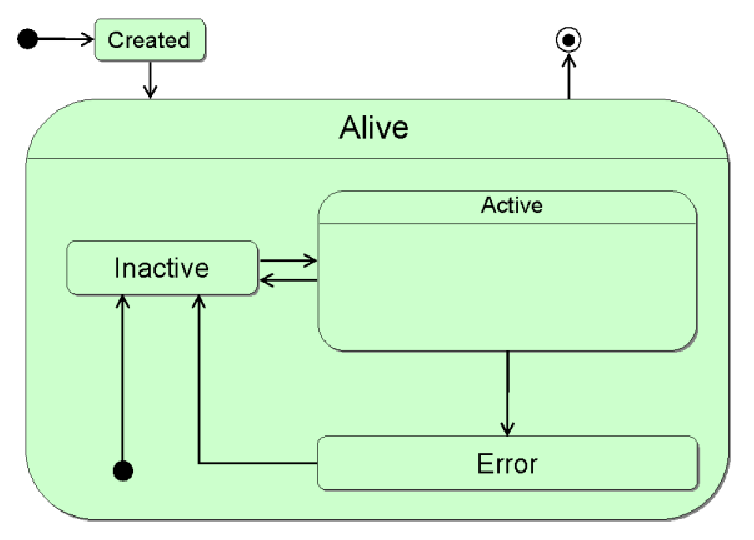
\includegraphics[width=58mm]{rtc-state.eps}
  \end{center}
  \caption{RTコンポーネントのステートチャート}
  \label{rtc-state.fig}
 \end{minipage}
\hfill
 \begin{minipage}{0.48\hsize}
  \begin{center}
   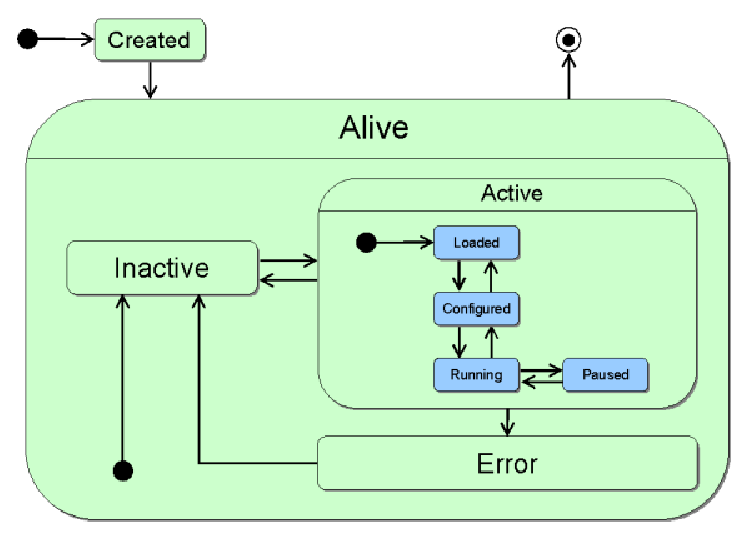
\includegraphics[width=58mm]{daq-state.eps}
  \end{center}
  \caption{DAQコンポーネントのステートチャート}
  \label{daq-state.fig}
 \end{minipage}
\end{figure}
 \begin{figure}[h]
   \vspace{-5mm}
  \begin{center}
   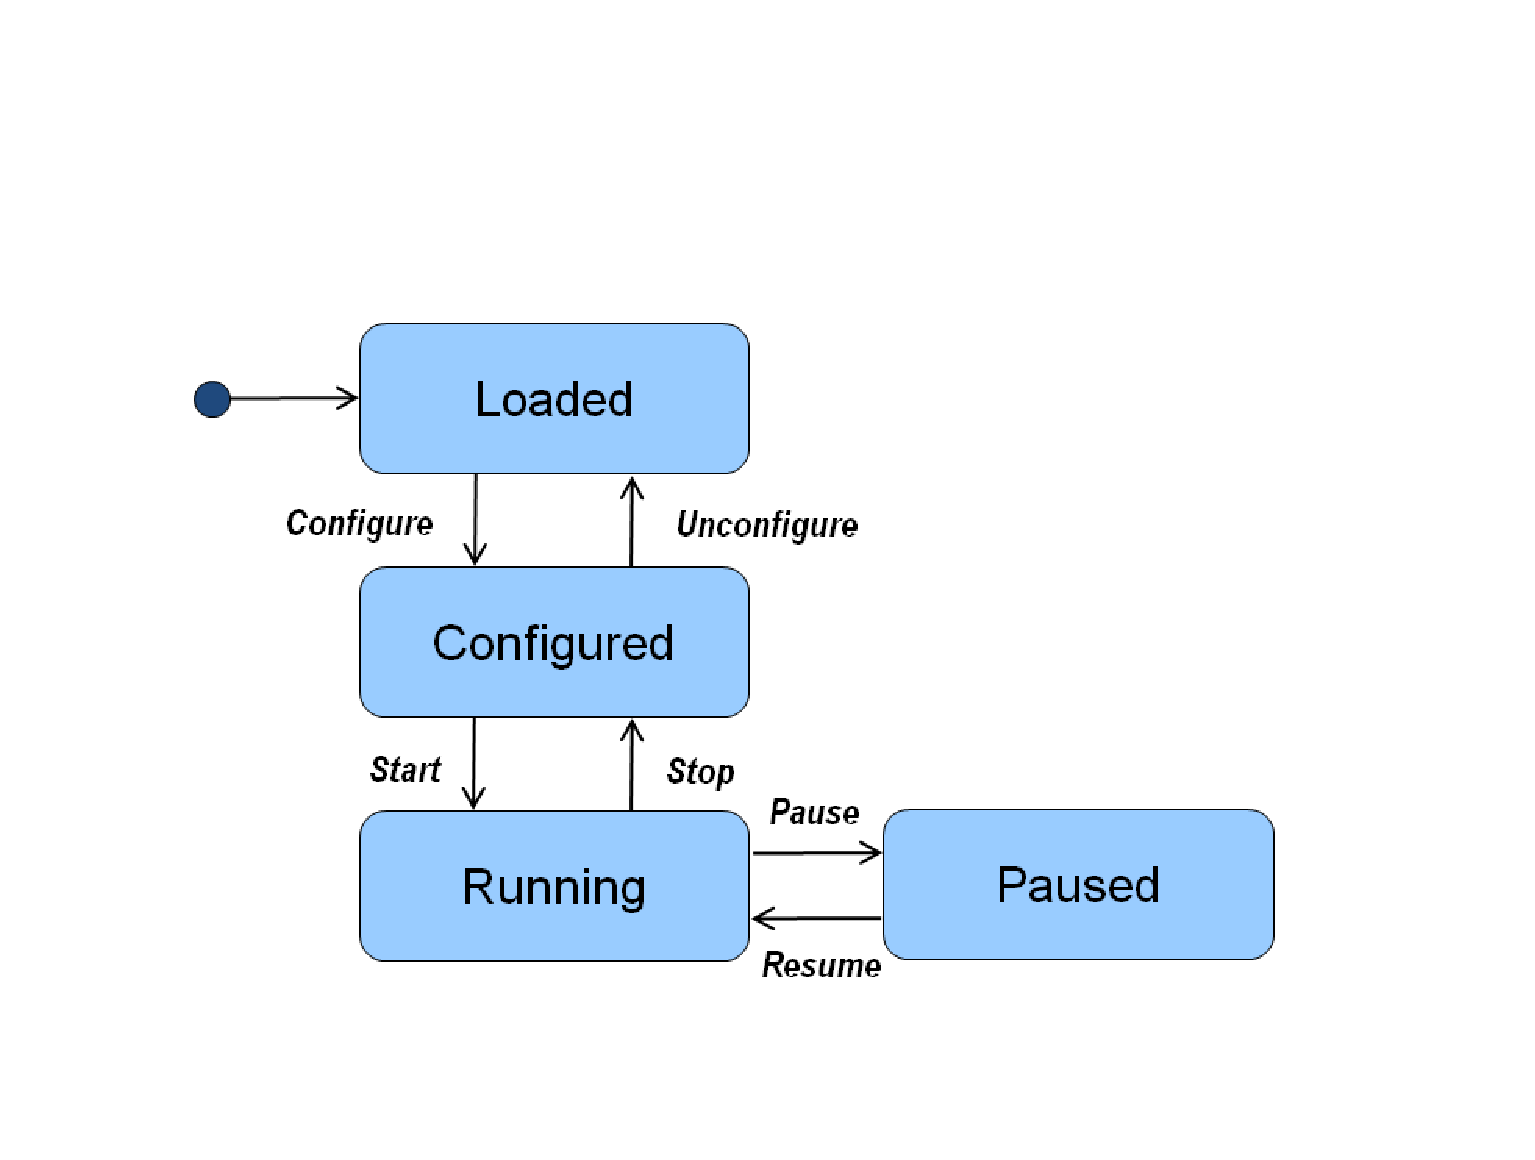
\includegraphics[width=100mm]{daq-state-only.eps}
   \vspace{-5mm}
   \caption{DAQコンポーネントのコマンドと状態遷移モデル}
  \label{command-state.fig}
  \end{center}
 \end{figure}

\subsection{ランコントロール・モデル}\label{runctrl}
現在のDAQミドルウェアのランコントロール・モデルは、1階層のツリー構造です。1つのDAQ
オペレータ(コントローラ)で、すべてのDAQコンポーネントを制御します。今後、より大規模な
システムに対応できるように、サブコントローラを導入し、多重階層化することも検討して
います。
前述のコンフィグレーション・ファイルでは、各DAQコンポーネントの起動の順番が記述します。
現在のDAQコンポーネント起動の順序は、それらを流れるデータストリームに
対して下流から起動を開始し、停止は上流から行うように実装されています。

\subsection{データ転送機能}\label{data-tarans}
DAQコンポーネント間のデータ転送は、RTコンポーネントのInPort, OutPortを使用します。
InPort, OutPortは、抽象化されたRTコンポーネントの通信インターフェイスで、データを
送受信するために作られたものです。DAQコンポーネント間は、同一ホスト中でもネットワーク
分散環境下でも透過的にデータ転送を行うことができます。
接続する際にデータポート間の通信手段を選択できます。
%%CORBAとsocketによるTCP 通信が選択可能で、
\daqmwcurrent では CORBA のみが選択可能です。次のリリースでは、
CORBA および socket によるTCP 通信の2つが選択可能になる予定です。socket を使ってデータ
転送を行なうことでCORBAに比べてオーバヘッドが減り、データ転送性能の向上が期待できます。

DAQコンポーネント間を流れるデータには8バイトのヘッダとフッタがついており、データの妥当性の
検証に使用します。

ヘッダには4バイトのマジック番号(0xe7e7)とデータのバイトサイズを4バイトで格納します。実際に取得したデータの
バイトサイズとヘッダに格納されているバイトサイズを比較することでデータの妥当性を検証できます。ヘッダには
予備として残り2バイトありますが、これはユーザが使用することができます。
フッターには4バイトのマジック番号(0xcccc)とシーケンス番号と呼ばれる4バイトの数値があります。シーケンス番号
は、コンポーネントの転送処理に応じて増加する値です。この数値によりデータに欠損がなかったか検証できます。
下記にヘッダとフッタのフォーマットを示します。

\begin{table}[h]
\begin{center}
\caption{ヘッダデータ}
\label{tbl:header}
\begin{tabular}{ l r l r l r l r l r l r l r l r}
\hline
\multicolumn{2}{|c|}{Header} & \multicolumn{2}{|c|}{Header} & \multicolumn{2}{|c|}{} & \multicolumn{2}{|c|}{} & \multicolumn{2}{|c|}{Event} & \multicolumn{2}{|c|}{Event} & \multicolumn{2}{|c|}{Event} & \multicolumn{2}{|c|}{Event} \\
\multicolumn{2}{|c|}{Magic}  & \multicolumn{2}{|c|}{Magic}  & \multicolumn{2}{|c|}{Reserved} & \multicolumn{2}{|c|}{Reserved} & \multicolumn{2}{|c|}{Byte Size} & \multicolumn{2}{|c|}{Byte Size} & \multicolumn{2}{|c|}{Byte Size} & \multicolumn{2}{|c|}{Byte Size}\\
\multicolumn{2}{|c|}{(0xe7)} & \multicolumn{2}{|c|}{(0xe7)} & \multicolumn{2}{|c|}{} & \multicolumn{2}{|c|}{} & \multicolumn{2}{|c|}{(24:31)} & \multicolumn{2}{|c|}{(16:23)} & \multicolumn{2}{|c|}{(8:15)} & \multicolumn{2}{|c|}{(0:7)}\\
\hline
0 & 7 & 8 & 15 & 16 & 23 & 24 & 31 & 32 & 39 & 40 & 47 & 48 & 55 & 56 & 63
\end{tabular}
\end{center}
%%\end{table}

%%\begin{table}[h]
\begin{center}
\caption{フッタデータ}
\label{tbl:footer}
\begin{tabular}{ l r l r l r l r l r l r l r l r}
\hline
\multicolumn{2}{|c|}{Footer} & \multicolumn{2}{|c|}{Footer} & \multicolumn{2}{|c|}{} & \multicolumn{2}{|c|}{} & \multicolumn{2}{|c|}{Sequence} & \multicolumn{2}{|c|}{Sequence} & \multicolumn{2}{|c|}{Sequence} & \multicolumn{2}{|c|}{Sequence} \\
\multicolumn{2}{|c|}{Magic}  & \multicolumn{2}{|c|}{Magic}  & \multicolumn{2}{|c|}{Reserved} & \multicolumn{2}{|c|}{Reserved} & \multicolumn{2}{|c|}{Number} & \multicolumn{2}{|c|}{Number} & \multicolumn{2}{|c|}{Number} & \multicolumn{2}{|c|}{Number}\\
\multicolumn{2}{|c|}{(0xcc)} & \multicolumn{2}{|c|}{(0xcc)} & \multicolumn{2}{|c|}{} & \multicolumn{2}{|c|}{} & \multicolumn{2}{|c|}{(24:31)} & \multicolumn{2}{|c|}{(16:23)} & \multicolumn{2}{|c|}{(8:15)} & \multicolumn{2}{|c|}{(0:7)}\\
\hline
0 & 7 & 8 & 15 & 16 & 23 & 24 & 31 & 32 & 39 & 40 & 47 & 48 & 55 & 56 & 63
\end{tabular}
\end{center}
\end{table}

\subsection{コマンド・ステータス通信}\label{status}
DAQコンポーネントとそのコントローラであるDAQオペレータの通信はサービスポートを使用して
います。前述のようにサービスポートはInPortやOutPortとは異なり、ユーザが任意のサービ
スインターフェースを定義できるポートです。
サービスポートは「サービスプロバイダ」、「サービスコンシューマ」モデルによりCORBAで
実装されています。
DAQコンポーネントは「サービスプロバイダ」で、DAQオペレータは「サービスコンシューマ」に
対応します。DAQコンポーネントのコントローラであるDAQオペレータからの要求(コマンド)
によりDAQコンポーネントは、その状態を遷移させます。
サービスのインターフェイスを定義するためにIDL(Interface Definition Language)を
使用します。
DAQミドルウェアでは、DAQService.idl というファイルにインターフェイスの定義があります。

\subsection{システム・コンフィグレーション}\label{config}
DAQミドルウェアでは、複数のDAQコンポーネントを自由に接続してデータ収集システムを構築
できます。それらのDAQコンポーネントはローカル計算機あるいはリモート計算機上で動いて
いても同様です。
このように使用するDAQコンポーネントの構成、それらの接続の仕方を決めることを
コンフィグレーションと呼んでいます。
その情報はコンフィグレーション・ファイル(config.xml)というXML文書により記述します。
XMLは現在、広く普及している技術で、構造化された文書やデータを異なる情報システム間で
共有できます。
コンフィギュレーション・ファイルの内容を変更することで、使用するDAQコンポーネント
を選択しコンポーネント間の接続を変更して柔軟にDAQシステムの変更が可能です。
このようにコンフィグレーションファイルはDAQシステムを記述する広義のデータベースと
しての意味を持ちます。
XML文書の文書構造をスキーマ言語により定義することができ、XML文書の構造の妥当性の検証に使用します。
コンフィグレーション・ファイルのスキーマ(config.xsd)はW3CのXML Schema で記述されています。
コンフィグレーション・ファイルにはDAQコンポーネントを起動する計算機のIPアドレス、
DAQコンポーネントの名前、使用するデータ入出力ポートの種類と名前、起動順番等を記述します。
DAQオペレータは、コンフィグレーション・ファイルを解釈して必要なDAQコンポーネントを
ネットワーク上から探して、コマンド・ステータス通信のため自身のサービスポートとDAQコンポー
ネントのサービスポートを接続します。また、config.xml の記述にしたがいDAQコンポーネント間
のデータ入力ポートと対応するデータ出力ポートを接続してデータストリームの経路を確立します。

詳細は\ref{operator-config}で説明します。


\subsection{システム・インターフェイス}\label{sysint}
システム・インターフェイスとは、DAQミドルウェアと外部システムを接続する際に用いる
インターフェイスです。
システム・インターフェイスは、より一般的な通信プロトコルを用いることが望ましいという
理由で XML データをHTTPで転送する方式を採用しています。
このプロトコルによる通信であれば、どのような言語、アプリケーションであっても
システムインターフェイスを介してランの制御が可能です。
例えば WebブラウザからDAQオペレータへコマンドを送信してランコントロールをすることも可能です。
J-PARC MLF中性子実験においては上位のシステムである「ソフトウェア・フレームワーク」と
このプロトコルを用いてDAQミドルウェアによるデータ収集システム・サブシステムと
通信を行っています。
\begin{figure}[htbp]
  \begin{center}
   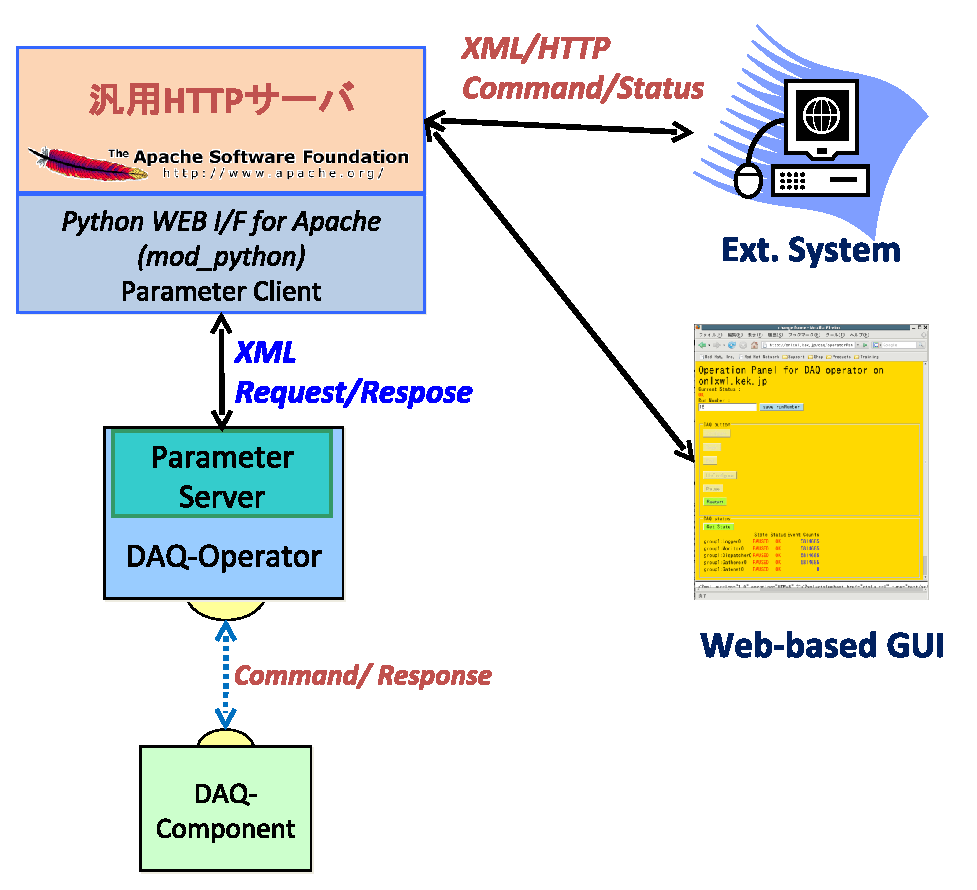
\includegraphics[width=100mm]{web-interface.eps}
  \end{center}
  %\vspace{-2mm}
  \caption{システム・インターフェイスの概念図}
  \label{web-interface.fig}
\end{figure}

%%その具体的な内容は参考文献 \cite{Web-GUI}の巻末の「参考資料」をご覧ください。
システム・インターフェイス機能の概念図を図 \ref{web-interface.fig}に示します。
DAQオペレータの"Webモード"では汎用HTTPサーバ(Apache)と通信するための
"Parameter Server"が起動します。
このサーバは\verb|mod_python|により実装された
"Parameter Client"からの要求を待ち受けています。\verb|mod_python|は、Apache で
Python を実行するためのモジュールです。
付録\ref{xmlhttp}に外部システムとの通信で使用するプロトコルの詳細を示します。

\subsection{装置および解析パラメータ設定機能}\label{cond}
前述のコンフィグレーション・ファイルとは別に装置パラメータやオンライン解析パラメータ情報
の広義のデータベースとしてXMLで書かれたコンディション・ファイルがあります。
コンフィグレーション・ファイルには実験のラン毎には変化しないDAQシステムの構成等の情報を
記述し、コンディション・ファイルにはラン毎に変化しうる、実験装置のパラメータやオンライン
解析用のパラメータ等を記述します。コンディション・ファイルの詳細は\ref{comp-cond}で説明
します。
コンフィグレーション・ファイルはDAQオペレータが読み込んで情報を取得しますが、コンディション・
ファイルは各コンポーネントが各自それを読み込んで必要な情報を取得します。
現在は、各コンポーネントでの XML構文解析処理の負荷を軽減するため、XML に比べて処理が軽量な 
JSON(JavaScript Object Notation)形式に変換したファイルを各コンポーネントが読み込んで処理を
行う方式をとっています。
図\ref{condition.fig}にコンフィグレーション・ファイルとコンディション・ファイルについて
、それぞれの役割を示します。
\begin{figure}[htbp]
%%\begin{wrapfigure}{r}{65mm}
 \begin{center}
  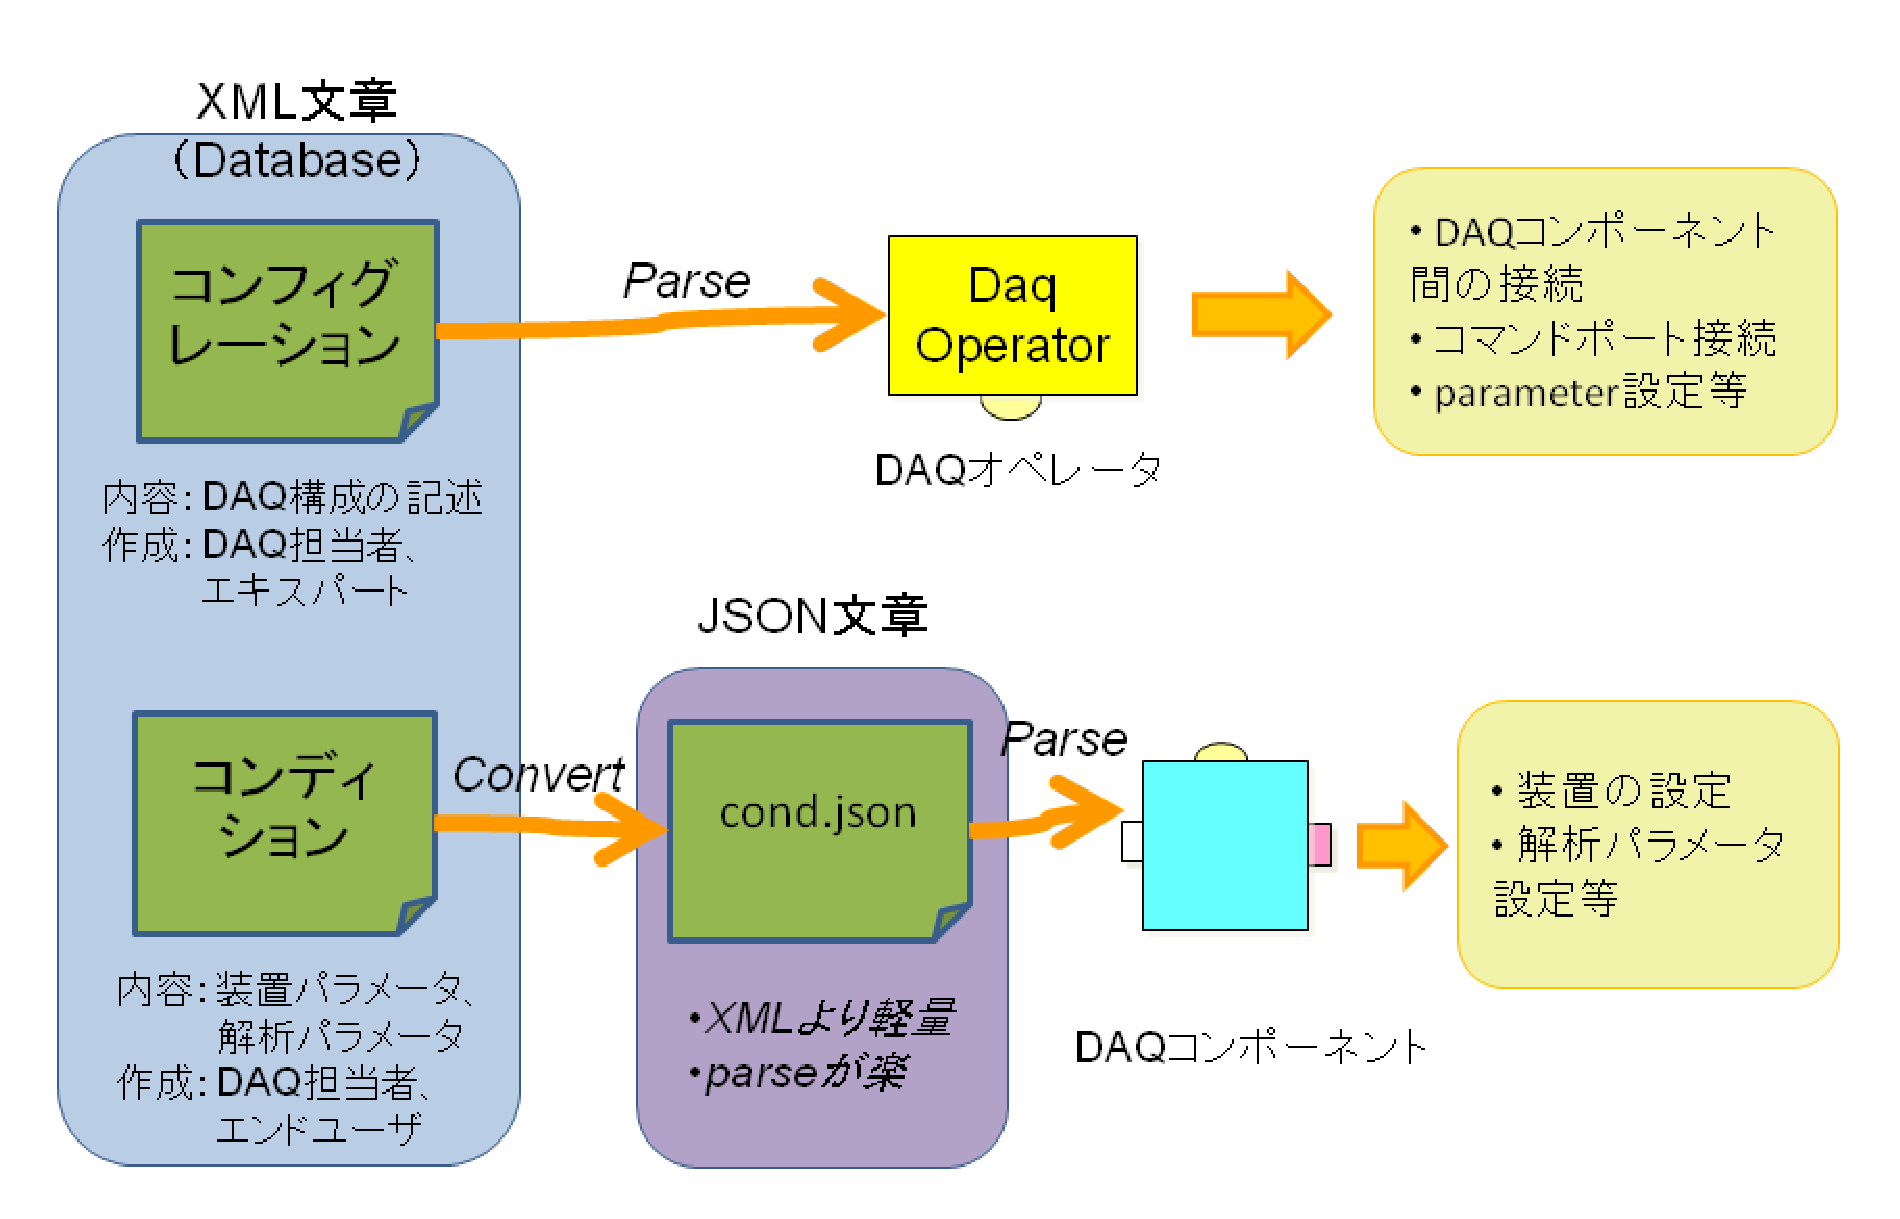
\includegraphics[width=90mm]{condition.eps}
  \caption{コンフィグレーション・ファイルとコンディション・ファイル}
  \label{condition.fig}
 \end{center}
\end{figure}
%%\end{wrapfigure}

\subsection{リモートブート機能}\label{remoteboot}
DAQミドルウェアのリモートブート機能とは、ネットワーク上の計算機(CPU DAQ)にあるDAQコンポーネントを
ローカル計算機(CPU UI)からのコマンドにより起動させる機能です。
具体的には、Linux xinetd のサービスのひとつとしてポート50000番に対して動作を行います。
J-PARC MLF中性子におけるリモートブートの利用例を図\ref{remote-booting.fig}に示します。
DAQシステム起動スクリプト run.py を起動します。
各コンポーネントの起動メカニズムを図\ref{remote-booting.fig}をもとに解説します。
\begin{enumerate}
\item ユーザーがローカル計算機のコマンドプロンプトから\url|run.py|を起動します。
  \url|run.py|はまず、各コンポーネントがネームサーバーと通信するのに
  必要となる情報が書かれたファイル\url|rtc.conf|を作成し、各リモート
  計算機にネットワークを通じて\url|rtc.conf|を送ります。リモート計算機側では
  このファイルを受信するためにxinetdから起動される受信サーバー
  \url|bootComps.py|を使います。受信したファイルは\url|/tmp/rtc.conf|
  に保存されます。なお\url|rtc.conf|の内容は各リモート計算機の
  構成にマッチしている必要があります。
\item \url|run.py|は続いてコンポーネント起動用スクリプト\url|run-comps.sh|
  ファイルを各リモート計算機に送ります。リモート計算機側では\url|rtc.conf|ファイル
  と同様にxinetdから起動された受信サーバー\url|bootComps.py|を使って
  \url|run-comps.sh|を受信します。受信したファイルは\url|/tmp/run-comps.sh|
  として保存されます。
\item xinetdから起動された\url|bootComps.py|は、\url|run-comps.sh|を受信後
  \url|/tmp/run-comps.sh|を\url|system()|関数で実行します。これで各コンポーネント
  が起動します。
\item 起動したコンポーネントは\url|/tmp/rtc.conf|を参照し、そこに書かれた
  情報をもとにNaming serviceへ自身を登録します。
\item 
  全てのリモート計算機へコンポーネントの起動をリクエストした後、
  \url|run.py|からDaqOperatorが起動されます。
\item 起動したDaqOperatorはローカルにある\url|config.xml|をパーズし、必要
  なコンポーネントをNaming serviceへ問い合わせ、コンポーネントを
  検索し、各コンポーネント間を接続します。Naming service に問い合わせて
  目的のコンポーネントが見つからない場合は、0.5秒スリープして20回のリトライ
  を行ないます。20回のリトライでコンポーネントが見つからない場合は、エラー
  となり、コンポーネントの起動に失敗します。すべてのコンポーネントが見つかった場合は、
  各コンポーネント間のデータポートが接続されデータ収集レディ状態になります。
\end{enumerate}

\begin{figure}[t]
  \centering
  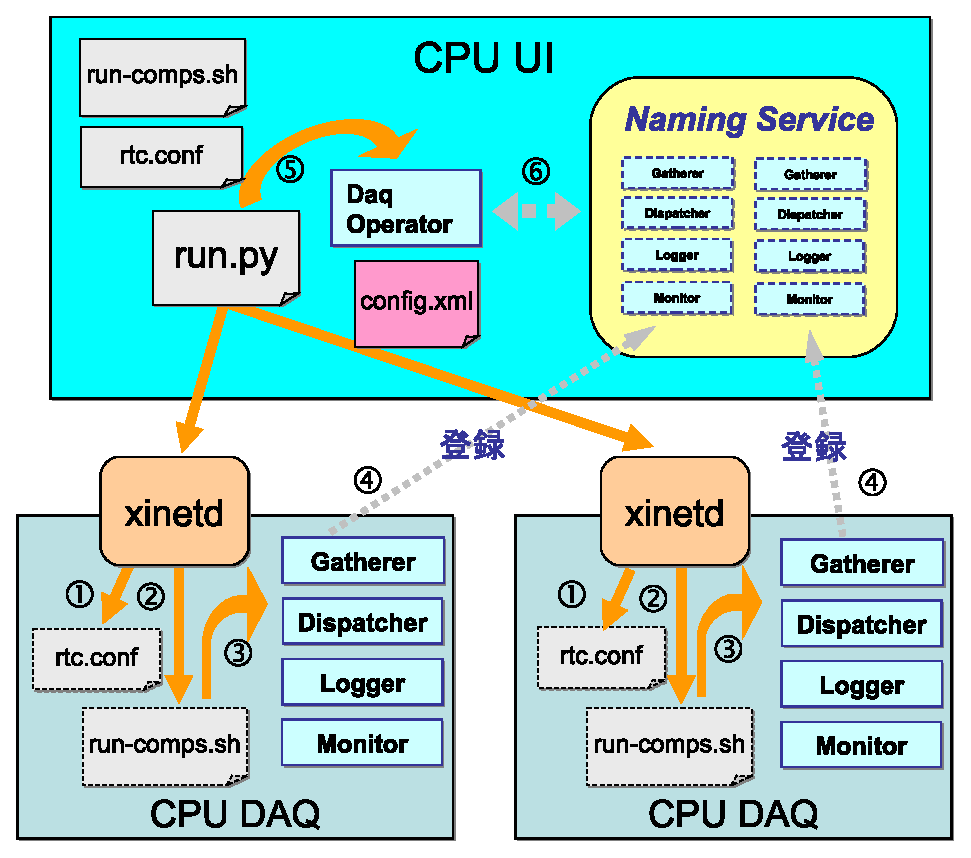
\includegraphics[scale=0.7]{boot.eps}
  \caption{DAQコンポーネントのリモート起動メカニズム。}
  \label{remote-booting.fig}
\end{figure}

%%%%%%%%%%%%%%%%%%%%%%%%%%%%%%%%%%%%%%%%%%%%%%%%%%%%%%%%%%%%%%%%%%%%%%%%%%%%%%%%%%%%%%%%%%%%%%%%%%

\section{DAQコンポーネントの仕様}\label{daqcomp}

\subsection{DaqComponentBaseクラス}
\verb|DaqComponentBase|クラスは、各DAQコンポーネント共通の機能の実装のために導入されました。
DAQミドルウェアではユーザが独自のDAQコンポーネントを開発してそれらを接続し、
DAQシステムを構築します。
新たなDAQコンポーネントを開発する際は、この\verb|DaqComponentBase|クラスを継承して
新たなクラスを作ります。この継承によりDAQコンポーネントとして必要とされる機能は、
実装されることになります。しかし継承しただけでは、何もしない(ロジックが空の)
DAQコンポーネントができるので、開発者は、各状態での動作の実装を行うことで
必要な機能を実現することができます。詳細は\ref{trans}で説明します。
DAQコンポーネントを開発するユーザは、各状態および状態遷移の実装のみ行なえばよいので、開発効率、
ソースコードのメンテナンスビリティの向上が図られます。

\verb|DaqComponentBase|クラスは、図\ref{class-diag.fig}のような継承関係を持っています。
データフロー型のRTコンポーネントは、\verb|RTC::DataFlowComponentBase| を継承して実装します。
DAQコンポーネントはデータフロー型RTコンポーネントから拡張して作られているので、
図\ref{class-diag.fig}のような継承関係があります。
DAQコンポーネントを開発する際は、\verb|DAQMW::DaqComponentBase| を継承して実装します。
\begin{figure}[htbp]
%%\begin{wrapfigure}{r}{65mm}
 \begin{center}
  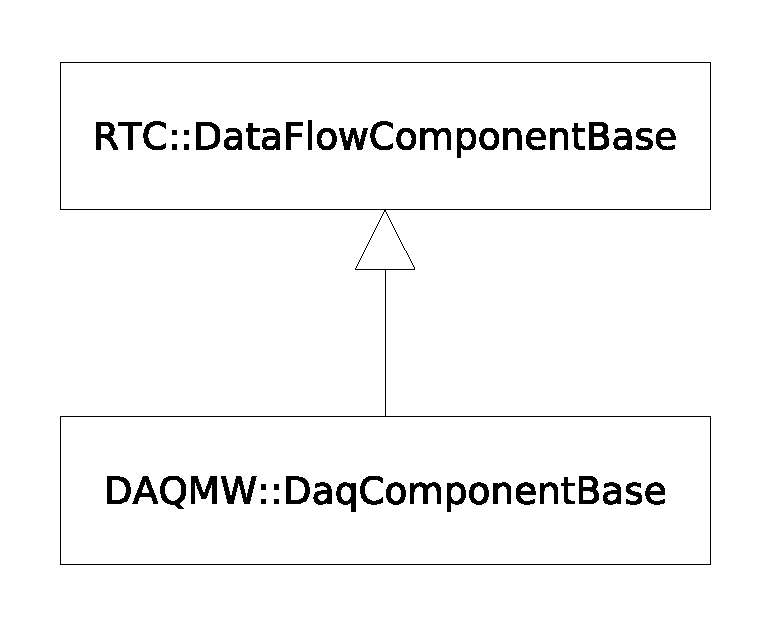
\includegraphics[width=60mm]{class-diag.eps}
  \caption{DAQコンポーネントのクラス図}
  \label{class-diag.fig}
 \end{center}
\end{figure}
%%\end{wrapfigure}

\verb|DaqComponentBase|クラスで実現している機能は次のものです。
\begin{itemize}
\item DAQのための状態遷移機能
\item コマンド受信/ステータス送信機能
\item Fatalエラーの際のステータス送信機能
%%\item イベント数等のメンバ変数
\end{itemize}

\verb|DaqComponentBase|クラスを継承して使用できるメンバ関数について説明します。
その一覧を付録\ref{funclist}に示します。

%%\begin{itemize}

\subsubsection{コンポーネント初期化}\label{init}
コンポーネントのコンストラクタで使用する関数として、コマンドポートの初期化を行なう\verb|init_command_port()|
, 状態遷移テーブルの初期化を行なう\verb|init_state_table()|, コンポーネントの名前を設定する\verb|set_comp_name()|があります。
\begin{Verbatim}
  int init_command_port()                コマンドポート初期化
  void init_state_table()                状態遷移テーブル初期化
  int set_comp_name(char* name)          コンポーネント名の設定
\end{Verbatim}

\subsubsection{シーケンス番号}\label{seq}
DAQコンポーネントはシーケンス番号と呼ばれる値を持っています。これは、データの入出力を行なうコンポーネントが
期待される処理を行った際に1づつ増やされる値です。例えば、検出器からデータを取得する
リーダコンポーネントは、データを取得しそのデータにヘッダとフッタをつけ、後段のコンポーネントに送信が成功した
場合に1つ増加させます。コンポーネントの処理の完了はコンポーネント開発者が知っているので、処理が完了したら
\verb|inc_sequence_num()|を使用します。またシーケンス番号のリセットや取得するためには下記の関数を使います。
\begin{Verbatim}
  int inc_sequence_num()                 シーケンス番号を1つ増加させる
  int reset_sequence_num()               シーケンス番号を0にする
  unsigned long long get_sequence_num()  シーケンス番号を取得する
\end{Verbatim}

\subsubsection{転送データサイズ}\label{datasize}
データの入出力を行なうDAQコンポーネントは、これまで自身が受信(または送信)したデータの総バイト数を持っています。
データストリームのスタートポイントとなるコンポーネントからエンドポイントとなるコンポーネントまで、その
値は等しくなることが要請されます(その間にデータをサンプリングしたりフィルタリングするコンポーネントが存在しない場合)。
転送データサイズのインクリメント、リセット、取得を行なうためには下記の関数を使います。
\begin{Verbatim}
  int inc_total_data_size(unsigned int byteSize) 指定したバイト数を総データバイト数に加える
  int reset_total_data_size()                    総バイト数を0にする
  unsigned long long get_total_data_size()       総バイト数を取得する
\end{Verbatim}

\subsubsection{データヘッダ、フッタ関連}\label{header}
\ref{data-tarans}で説明したヘッダ情報、フッタ情報をセットする関数として次の2つが用意されています。
データバイト数をヘッダに格納する\verb|set_header()|、シーケンス番号をフッタにセットする\verb|set_footer()|です。
データバイト数やシーケンス番号は、データを受信した際にデータの妥当性の検証に使用します。
\begin{Verbatim}
  int set_header(unsigned char* header, unsigned int data_byte_size) ヘッダにデータバイト数を格納
  int set_footer(unsigned char* footer, unsigned int sequence_num)   フッタにシーケンス番号を格納
\end{Verbatim}

ヘッダ情報、フッタ情報をチェックするための関数として次の3つがあります。\verb|check_header(), check_footer()|では
チェックした結果が bool 値で返るので、ユーザはその値が False だった場合は、\verb|fatal_error_report()| を呼んでFatalエラー
を報告し、自身はアイドル状態になります。
\verb|check_header_footer()|では、ヘッダまたはフッタに問題がある場合は、その関数中で\verb|fatal_error_report()| を
呼んでいます。

\begin{Verbatim}
  bool check_header(unsigned char* header, unsigned received_byte)     ヘッダのチェックを行なう
  bool check_footer(unsigned char* footer, unsigned loop_cnt)          フッタのチェックを行なう
  bool check_header_footer(const RTC::TimedOctetSeq& in_data, unsigned int block_byte_size) 
  上記の2つを行なう
\end{Verbatim}

\verb|get_event_size()|は与えられたデータのバイト数からヘッダとフッタを除いた正味のデータバイト数を返します。
\begin{Verbatim}
  unsigned int get_event_size(unsigned int block_byte_size)  正味のデータ数を取得する
\end{Verbatim}

\subsubsection{状態遷移関連}\label{state}
\verb|DaqComponentBase| 中では、ストップコマンドを受信するとRUNNING状態からCONFIGURED状態への遷移
(状態遷移に関しては\ref{trans}で説明)がロックされます。
なぜならコンポーネントが安全にCONFIGURED状態に遷移するためには、現在処理中の動作を完了する必要があるからです。
処理の完了の定義はコンポーネントによって違うので、そのロックを解除するのはコンポーネント自身です。
具体的には、\verb|daq_run()|中の中断可能なポイントでストップコマンドの有無を確認する\verb|check_trans_lock()|を呼んで、
その返り値が真の場合は、\verb|set_trans_unlock()|を呼び、次の状態に遷移可能であることを知らせます。

\begin{Verbatim}
  bool check_trans_lock()  ストップコマンドが発行されているかチェックする
  void set_trans_unlock()  RUNNING状態からCONFIGURED状態へ遷移を行なう
\end{Verbatim}

\subsubsection{致命的(Fatal)エラー処理関連}\label{fatal}
DAQコンポーネントはユーザがその目的に応じて自由に開発できます。したがって
DAQコンポーネントでは、種々のエラーが起こる可能性があります。DAQミドルウェアではFatalエラーは、「エラーが起きた場合そのコンポーネント
自身で解決できないもの」と定義しています。その場合、下記の関数を呼んでDAQオペレータに報告し、自身はアイドル
状態になります。Fatal エラーの情報を受信したユーザ(人)または上位のフレームワークでは、ランをストップします。
Fatalエラー後の処理として一般的には、ストップコマンドによりランをストップして、そのエラーの原因を取り除いて、再スタートするか
全コンポーネントを終了して再起動するかのどちらかです。
%% これは各コンポーネントのロジックや実装、運用に依存します。例えば、「あるエラーが起きたが
%% 5回リトライ後に正常に終了した」場合等は、Fatalエラーとしない場合もあるでしょうが、「そのエラーが起きた時点でリトライはしない」
%% 場合は、Fatalエラーになりえます。開発者や実験のポリシーにより Fatal エラーは定義されると考えています。
DAQミドルウェアでは、Fatal エラーのタイプとしてDAQミドルウェアで定義しているものと、ユーザが定義するものの2つに分類しています。
詳細は\ref{fatal_error}で説明します。DAQミドルウェアで定義済のエラーは enum でその種類を指定します。ユーザによる定義のもの
は、enum として \verb|USER_DEFINED_ERROR1,...,USER_DEFINED_ERROR20|から他のエラーと重複しないように指定して、エラーの詳細を
文字列で指定します。これは、上位のフレームワークでユーザ定義の enum に対応した処理を行なう場合に
有効です。

\subsubsection{転送ステータス取得}\label{portstat}
DAQ-Middleware 1.0.0では、下記の関数でデータポートのステータスを取得できます。
\begin{Verbatim}  
  BufferStatus check_outPort_status(RTC::OutPort<RTC::TimedOctetSeq> & myOutPort) 
  指定した OutPort の転送ステータスを取得する

  BufferStatus check_inPort_status(RTC::InPort<RTC::TimedOctetSeq> & myInPort)
  指定した InPort の転送ステータスを取得する    
\end{Verbatim}
返り値のBufferStatus は、次のようなenum です。
\begin{Verbatim}
  enum BufferStatus {BUF_FATAL = -1, BUF_SUCCESS, BUF_TIMEOUT, BUF_NODATA, BUF_NOBUF}
\end{Verbatim}

DAQ-Middleware 1.0.0では、下記の関数でデータポートの接続を確認できます。例えばCONFIGURED状態からRUNNING状態へ
遷移する際に、\verb|daq_start()| 中で呼んでデータポートの接続を確認して、\verb|daq_run()|でデータの転送を行ないます。
\begin{Verbatim}  
  bool check_dataPort_connections(RTC::OutPort<RTC::TimedOctetSeq> & myOutPort)
  OutPortの接続を確認

  bool check_dataPort_connections(RTC::InPort<RTC::TimedOctetSeq> & myInPort)
  InPortの接続を確認
\end{Verbatim}

\verb|DaqComponentBase| クラスを継承して作るDAQコンポーネントは、下記の状態遷移に関係する下記の
仮想関数を実装する必要があります。どのように実装するかは\ref{trans}で説明します。

\begin{Verbatim}
  ...
  virtual int daq_dummy() = 0;
  virtual int daq_configure()   = 0;
  virtual int daq_unconfigure() = 0;
  virtual int daq_start() = 0;
  virtual int daq_run()   = 0;
  virtual int daq_stop()  = 0;
  virtual int daq_pause() = 0;
  virtual int daq_resume()= 0;
  ...
\end{Verbatim}

%%\end{itemize}

%% \subsection{状態遷移モデル}
%% DAQシステムの状態遷移モデルとして、我々は"LOADED", "CONFIGURED", "RUNNING", "PAUSED"という4つの状態
%% によるランコントロールを行っています。状態の追加または削除も原理的には可能ですが、\verb|DaqComponentBase|
%% 自体の変更が必要になります。
%% RTコンポーネントでは、"Active", "Inactive","Error" の3つの状態が定義されています。我々は、上記の
%% DAQコンポーネントの4つの状態を図のようにRTコンポーネントの"Active"状態へマッピングを行いました。
%% \begin{figure}[htbp]
%%  \begin{center}
%%   \includegraphics[width=100mm]{state-rtc-daq.eps}
%%   \caption{\footnotesize ステートチャート}
%%   \label{state-rtc-daq.fig}
%%  \end{center}
%% \end{figure}

\subsection{DAQコンポーネントのファイル構成}
DAQコンポーネント開発に必要なファイルについて説明します。
例えば、Skeleton という名前のコンポーネントを開発するためには、次のファイルが必要です。
これはRTコンポーネントのファイル構成に由来するものです。
\begin{itemize}
\item Skeleton.h
\item Skeleton.cpp
\item SkeletonComp.cpp
\item Makefile
\end{itemize}

Skeleton.h は、Skeletonクラスのヘッダファイルです。
Skeleton.cpp にはSkeletonコンポーネントの各状態でのロジックを実装します。詳細は
\ref{trans}で説明します。
SkeletonComp.cpp は、Skeletonコンポーネントのメインプログラムです。
下記にその一部分を示します。RTC::Manager はRTコンポーネントの情報管理を行うクラスです。
\begin{itemize}
\item \verb|manager->init(argc, argv)|によりconfigファイルの読み込み、Naming Service の
  初期化等を行います。
\item \verb|manager->setModuleInitProc(MyModuleInit)|によりコンポーネントの初期化
プロシージャが設定されます。
\item \verb|manager->activateManager()|によりコンポーネントの生成を行います。
\item \verb|manager->runManager()|でマネージャのメインループを実行します。 このメイン
ループ内では、CORBA ORBのイベントループ等が処理されます。デフォルトでは、
このオペレーションはブロックします。
\end{itemize}

\begin{Verbatim}
  int main (int argc, char** argv)
  {
      RTC::Manager* manager;
      manager = RTC::Manager::init(argc, argv);
      
      // Initialize manager
      manager->init(argc, argv);

      // Set module initialization proceduer
      // This procedure will be invoked in activateManager() function.
      manager->setModuleInitProc(MyModuleInit);
    
      // Activate manager and register to naming service
      manager->activateManager();

      // run the manager in blocking mode
      // runManager(false) is the default.
      manager->runManager();

      // If you want to run the manager in non-blocking mode, do like this
      // manager->runManager(true);

      return 0;
  }
\end{Verbatim}

\subsection{状態および状態遷移の実装}\label{trans}
DAQコンポーネントの \verb|DaqComponentBase|クラスには、状態遷移の際に呼ばれるメンバ関数、
その状態中に繰り返し呼ばれるメンバ関数が定義されています。DAQコンポーネント開発者は、
それらの関数の中を実装して新しい機能のDAQコンポーネントを作ります。

図 \ref{state-func.fig}に状態遷移の際に呼ばれるメソッド、その状態中に繰り返し呼ばれる
メソッドを示します。また状態遷移のトリガとなるコマンドを示します。
コマンドは、DAQService.idl に次のように enum で定義されています。
\begin{Verbatim}
  enum DAQCommand
  {
      CMD_CONFIGURE,
      CMD_START,
      CMD_STOP,
      CMD_UNCONFIGURE,
      CMD_PAUSE,
      CMD_RESUME,
      CMD_NOP
  };
\end{Verbatim}
また、コマンドに対応する状態は、次のように enum で定義されています。
\begin{Verbatim}
  enum DAQLifeCycleState
  {
      LOADED,
      CONFIGURED,
      RUNNING,
      PAUSED
  };
\end{Verbatim}

\begin{enumerate}
\item DAQコンポーネントは起動時は、"LOADED" 状態で待機状態\\
  現在の実装では、"LOADED" 状態中は、\verb|daq_dummy()|が繰り返し呼ばれる。
  \verb|daq_dummy()|は
  CPUを消費しないようにsleep()関数を呼んでアイドル状態を実現している。

\item "LOADED" 状態中は"Configure"コマンドを受けて"CONFIGURED"状態へ遷移\\
  その際、\verb|daq_configure()|が一度呼ばれる。コンポーネントに対するパラメータの
  設定を行う。
  "CONFIGURED"状態では、\verb|daq_dummy()|が繰り返し呼ばれアイドル状態。

\item "CONFIGURED"状態中は"Start"コマンドで"RUNNING"状態へ遷移\\
  その際、\verb|daq_start()|が一度呼ばれる。コンポーネントが連続動作を行う前の初期化
  等の処理を実装する。
  "RUNNING"状態中は、\verb|daq_run()|が繰り返し呼ばれる。\verb|daq_run()|に
  コンポーネントの機能のロジックを実装する。

\item "RUNNING"状態中は"Pause"コマンドで"PAUSED"状態へ遷移\\
  その際、\verb|daq_pause()|が一度呼ばれる。コンポーネントが"PAUSED"状態へ遷移する前に
  行う処理を実装する。"PAUSED"状態では\verb|daq_dummy()|が繰り返し呼ばれアイドル状態。

\item "PAUSED"状態中は"Resume"コマンドで"RUNNING"状態へ遷移\\
  その際、\verb|daq_resume()|が一度呼ばれる。コンポーネントが"RUNNING"状態へ遷移する
  前に行う処理を実装する。

\item "RUNNING"状態中は "Stop"コマンドで"CONFIGURED"状態へ遷移\\
  その際、\verb|daq_stop()|が一度呼ばれる。コンポーネントが連続動作を終了するための
  処理等を実装する。

\item "CONFIGURED"状態中は"Unconfigure"コマンドで"LOADED"状態へ遷移します。
  その際、\verb|daq_unconfigure()|が一度呼ばれる。"CONFIGURED"状態中は
  \verb|daq_dummy()|が繰り返し呼ばれアイドル状態。
\end{enumerate}

\begin{figure}[htbp]
 \begin{center}
  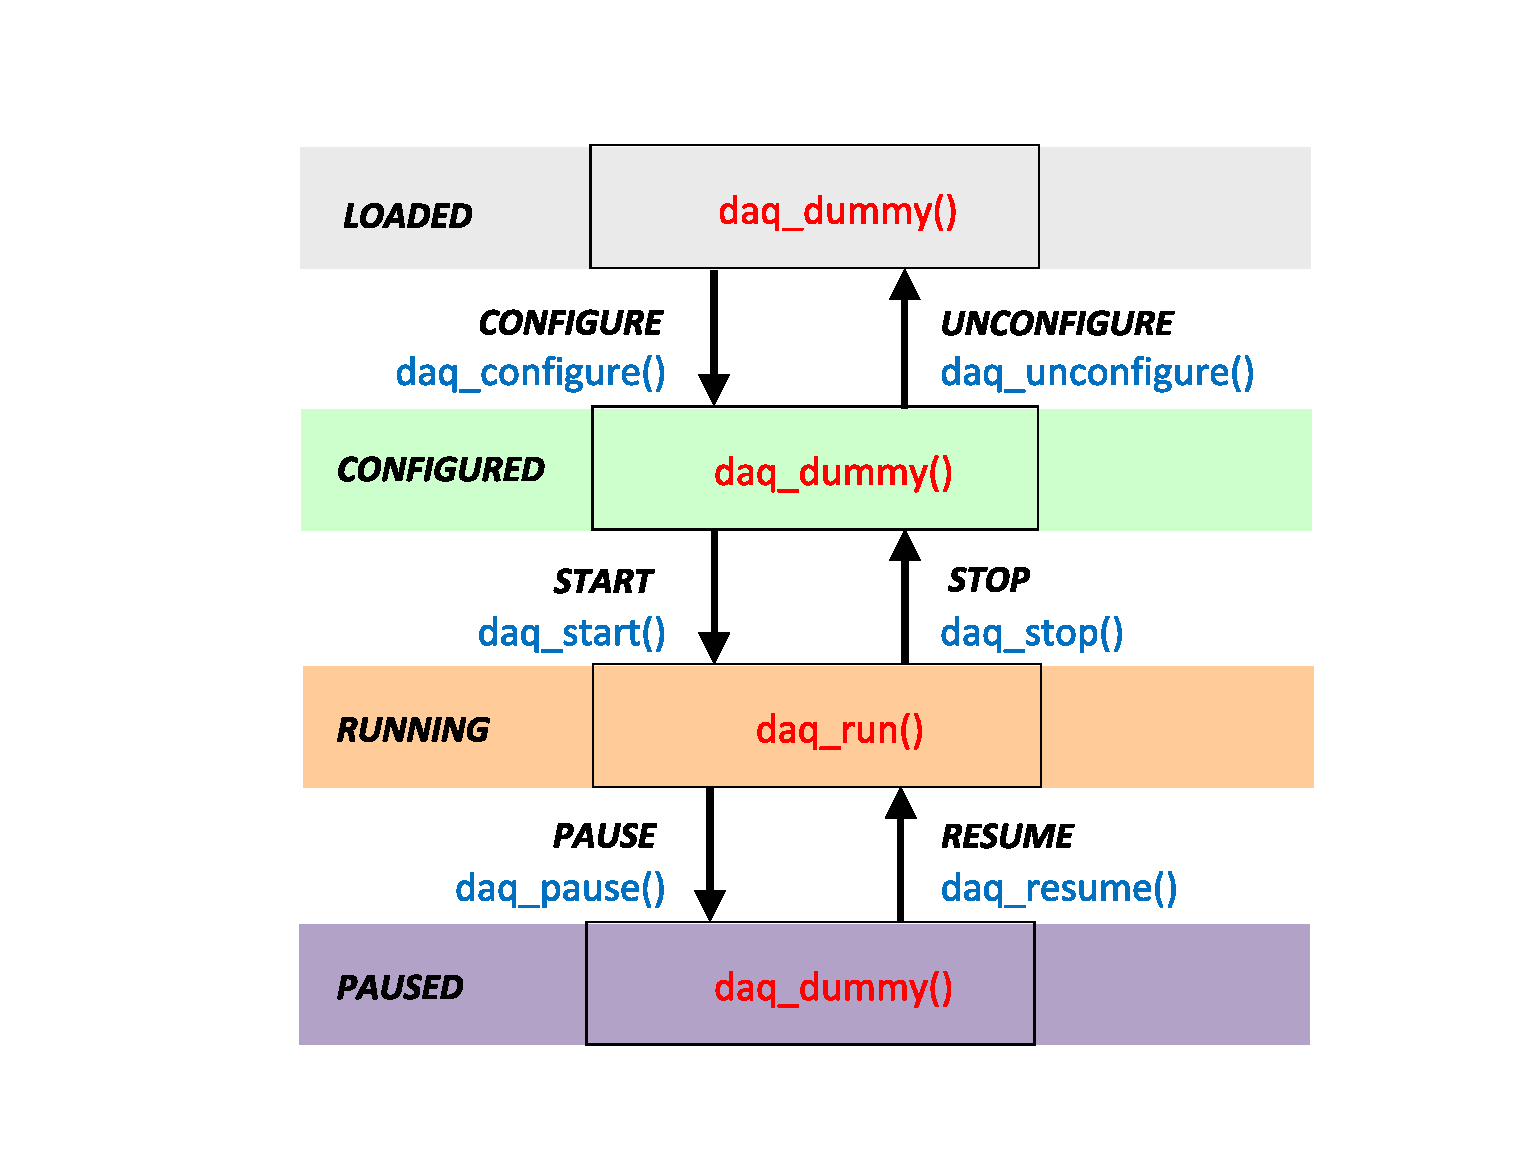
\includegraphics[width=100mm]{state-func.eps}
  \caption{DAQコンポーネントのステートチャート}
  \label{state-func.fig}
 \end{center}
\end{figure}

\subsubsection{RUNNING状態の動作の実装}
開発するDAQコンポーネントの機能(メインロジック)を実装します。例えば、次のような動作の
実装を行います。
\begin{itemize}
\item J-PARC MLFで仕様している Gathererコンポーネントは、リードアウト・モジュールから
  データを取得してデータにヘッダとフッタを付けて後段のコンポーネントへ送信する
\item Loggerコンポーネントは受信したデータからヘッダとフッタを取り除いてファイルへ保存する
\item Monitorコンポーネントは受信したデータをデコードして、興味のある物理量等を
  計算してヒストグラム化する
\end{itemize}

\subsection{コマンドの受信}
DAQオペレータから送信されるコマンドの受信は、\verb|DaqComponentBase::daq_do()|の中の 
\verb|get_command()|で行っています。これは前述のように、サービスポート間のデータ転送が
CORBAにより実現されています。現在のコンポーネントの状態(ステート)と受信したコマンド
により、状態遷移を行います。

\subsection{ステータスの送信}
DAQコンポーネントは各状態(例えば "RUNNING"状態)では定期的(2秒毎)に、下記の構造体のデータ
を自身のステータスとして更新します。具体的には、コンポーネントの名前、状態(ステート)、
イベント数、コンポーネントのサブ・ステータスです。
ある状態から別の状態へ遷移した場合または致命的なエラーが発生した場合は、ステータス情報は、
そのタイミングで更新されます。

\begin{Verbatim}
  struct Status
  {
      ComponentName comp_name;
      DAQLifeCycleState state;
      unsigned long long event_size;
      CompStatus comp_status;
  };
\end{Verbatim}

\subsection{データ送受信}
DAQコンポーネントは、任意の数のデータ入出力ポートを持つことができます。これはRTコンポーネント
から受け継いだ機能です。ユーザが開発を行なう機会が多いのは、データストリームの始点となる
ソース(source)タイプコンポーネントと終点となるシンク(sink)タイプコンポーネントです。
例えば検出器やリードアウトモジュールからデータを取得して、後段のコンポーネントに送信するのが
ソースタイプです。前段のコンポーネントからデータを受信して、ファイルに保存するコンポーネント
やデータをデコードしてヒストグラム等にしてオンラインモニタを行なうコンポーネントはシンクタイプ
です。

\subsubsection{データ受信}
InPort を持つコンポーネントはOutPortをもつコンポーネントからデータを受信できます。
InPort には関連付けられたリングバッファがあり、OutPortから送信されたデータはこのバッファに書き込まれ
ます。下記の \verb|read()| によりタイムアウト付きのブロックモードでデータを読み込みます。正常にデータが
読み込まれた場合は、返り値は \verb|true| になります。false の場合は、\verb|check_inPort_status()|により
転送ステータスを調べます。\verb|false| の場合、\verb|check_inPort_status()|は、\verb|BUF_TIMEOUT|または
\verb|BUF_FATAL|を返します。タイムアウトの場合はリトライを、Fatalの場合は、\verb|fatal_error_report()|
により報告します。

\begin{Verbatim}
  bool ret = m_InPort.read()
\end{Verbatim}

\subsubsection{データ送信}
OutPort を持つコンポーネントはInPortをもつコンポーネントへデータを送信できます。

下記の \verb|write()| によりタイムアウト付きのブロックモードでデータを書き込みます。正常にデータが
書き込まれた場合は、返り値は \verb|true| になります。false の場合は、\verb|check_outPort_status()|により
転送ステータスを調べます。\verb|false| の場合、\verb|check_outPort_status()|は、\verb|BUF_TIMEOUT|または
\verb|BUF_FATAL|を返します。タイムアウトの場合はリトライを、Fatalの場合は、\verb|fatal_error_report()|
により報告します。
\begin{Verbatim}
  bool ret = m_OutPort.write()
\end{Verbatim}

\subsection{致命的エラー報告の送信}\label{fatal_error}
DAQコンポーネントで、致命的な(Fatal)エラーが起きた場合は、
\verb|fatal_error_report()| という関数を呼んでDAQオペレータへFatal エラーを報告します。

\begin{Verbatim}  
  void fatal_error_report(FatalType::Enum type, int code = -1)
  void fatal_error_report(FatalType::Enum type, const char* desc, int code = -1)
\end{Verbatim}

DAQコンポーネント自身は、アイドル状態となり次のコマンドを待ちます。
これは各DAQコンポーネントで復旧不可能なエラーが発生した場合に、その情報を
DAQオペレータからユーザまたは上位システムに伝え、エラーの対応を行ってもらうためです。
例えば、"RUNNING"状態であれば、"Stopコマンド"によりランを停止する等です。
どのような状態をFatalエラーにするかは、コンポーネント開発者が自身で決めます。
下記のように、OutPort からデータを転送した後、そのステータスをチェックしてエラーの
場合は、 \verb|fatal_error_report()| を呼びます。
\begin{Verbatim}
  if (check_outPort_status(m_out_status) == -1) {
      std::cerr << "### EchoReader: OutPort.write(): FATAL ERROR\n";
      fatal_error_report(OUTPORT_ERROR);
  }
\end{Verbatim}

Fatalエラーのタイプは、FatalType.h で enum により下記のように定義してあります。

\begin{Verbatim}
  namespace DAQMW
  {
      namespace FatalType
      {
          enum Enum
          {
              ///DAQ-Middleware defined fatal error
              ///use following function
              ///fatal_error_report(FatalTypes types, int code)
              /// e.g. fatal_error_report(HEADER_DATA_MISMATCH, -1)

              ///header, footer error
              HEADER_DATA_MISMATCH,
              FOOTER_DATA_MISMATCH,
              SEQUENCE_NUM_MISMATCH,

              ///configuration file
              CANNOT_OPEN_CONFIGFILE,
              CONFIGFILE_PARSE_ERROR,
              NO_CONFIG_PARAMS,

              ///condition file
              CANNOT_OPEN_COND_FILE,
              COND_FILE_PARSE_ERROR,

              ///command/status path error
              CANNOT_CONNECT_COMMANDPATH,
              COMMANDPATH_DISCONNECTED,

              ///data path error
              CANNOT_CONNECT_DATAPATH,
              DATAPATH_DISCONNECTED,

              ///InPort/OutPort error
              INPORT_ERROR,
              OUTPORT_ERROR,
	      
              ///wrong parameters, such as command line options, etc.
              BAD_PARAMETER,
	      
              ///readout module-related error
              CANNOT_CONNECT_DATA_SRC,
              TOO_MANY_DATA_FROM_DATA_SRC,
              READOUT_ERROR,
	      
              ///file I/O error
              BAD_DIR,
              CANNOT_MAKE_DIR,
              CANNOT_OPEN_FILE,
              CANNOT_WRITE_DATA,
	      
              ///user defined fatal error (user defined error1 - error20)
              ///users can choose a below error and its description by string.
              ///fatal_error_report(FatalTypes types, std::string desc, int code)
              /// e.g. 
              /// fatal_error_report(USER_DEFINED_ERROR1,
              ///                                "My fatal error detail", -1)
              USER_DEFINED_ERROR1,
              USER_DEFINED_ERROR2,
              USER_DEFINED_ERROR3,
              USER_DEFINED_ERROR4,
              USER_DEFINED_ERROR5,
              USER_DEFINED_ERROR6,
              USER_DEFINED_ERROR7,
              USER_DEFINED_ERROR8,
              USER_DEFINED_ERROR9,
              USER_DEFINED_ERROR10,
              USER_DEFINED_ERROR11,
              USER_DEFINED_ERROR12,
              USER_DEFINED_ERROR13,
              USER_DEFINED_ERROR14,
              USER_DEFINED_ERROR15,
              USER_DEFINED_ERROR16,
              USER_DEFINED_ERROR17,
              USER_DEFINED_ERROR18,
              USER_DEFINED_ERROR19,
              USER_DEFINED_ERROR20,

              ///unknown error
              UNKNOWN_FATAL_ERROR
          };
  ...
\end{Verbatim}

現在、ユーザが使用できる CompFatalTypes は、\verb|USER_ERROR1|〜\verb|USER_ERROR20| の20個です。
1つのDAQコンポーネント中で最大20個のFatalエラーをユーザが定義できることになります。エラーの説明として
文字列を指定できます。
\begin{Verbatim}
  if (user_defined_fatal2) {
      std::cerr << "### MyComponent: FATAL ERROR\n";
      fatal_error_report(USER_DEFINED_ERROR2, "COULD NOT ACCESS READOUT MODULE");
  }
\end{Verbatim}

\subsection{装置パラメータ設定機能}\label{comp-cond}
DAQコンポーネントは、必要があれば装置パラメータやオンライン・モニタ用のパラメータを
コンディション・ファイルと呼ばれるXML文書から取得して、ランのスタート時に装置へ設定
することが可能です。
J-PARC MLF 中性子PSD検出器系のDAQシステムでは、NEUNETというリードアウト・モジュールに
対して、PSD検出器の信号のスレッショルド・レベルを設定する際に使用しています。
この機能をどのようにDAQコンポーネントに実装するかは、\cite{Cond-manual}を参照して
ください。

%%%%%%%%%%%%%%%%%%%%%%%%%%%%%%%%%%%%%%%%%%%%%%%%%%%%%%%%%%%%%%%%%%%%%%%%%%%%%%%%%%%%%%%%%%%%%%%%%%
\section{DAQオペレータの仕様}\label{daqop}
DAQオペレータは、DAQコンポーネントを制御するコンポーネントです。DAQオペレータは
次のような機能を持っています。
\begin{itemize}
\item コンフィグレーションファイル(XML文書)によるシステムコンフィグレーション機能
\item DAQコンポーネントへのコマンド送信/ステータス取得機能
\item 各DAQコンポーネントへのパラメータ送信機能
\item XML/HTTP プロトコルによる外部システムとのインターフェイス機能
\item 標準入力からのコマンドによるランコントロール
\end{itemize}

DAQオペレータは、ユーザまたは上位システムからコマンドを取得して、各DAQコンポーネント
へ通知するよう設計されています。テストまたはデバッグ用に標準入力からコマンドを取得して、
同様に各コンポーネントへコマンドを通知するモードもあります。この文章ではそれぞれ
「Webモード」、「コンソール・モード」と呼ぶことにします。
上記のその他の機能については後述します。

\subsection{コンフィグレーション機能}\label{operator-config}
\ref{config}で述べたように XML文書によるDAQシステムのコンフィグレーションが可能です。
XML文書には、次のようなDAQシステムの情報が記述されています。
\begin{itemize}
\item DAQオペレータのIPアドレス
\item 使用するDAQコンポーネントのIPアドレス
\item 使用するDAQコンポーネントのインスタンス名
\item 個々のDAQコンポーネントが使用する InPort, OutPortの名前
\item DAQコンポーネント間を流れるデータストリームを決めるための情報
\end{itemize}

システム・コンフィグレーションのシーケンスは次のようになっています。
\begin{enumerate}
\item DAQコンポーネントは起動後、RTコンポーネントの機能を使い自分自身のインスタンス名を 
  CORBA Naming Serviceへ登録します。
\item DAQオペレータは起動後コンフィグレーション・ファイルを読み込み構文解析を行います。
\item DAQオペレータは、コンフィグレーション・ファイルに記述されているDAQコンポーネントを
Naming Serviceへ問い合わせてそのオブジェクト・リファレンスを取得します。オブジェクト・
リファレンスとはCORBAオブジェクトを識別するために用いられる参照です。
\item DAQオペレータはそのオブジェクト・リファレンスを使って、DAQコンポーネントの
  ポート間の接続を行います。これによりコンポーネント間のデータストリームの経路が
  確立します。
\item DAQオペレータは自身のサービスポートと各DAQコンポーネントのサービスポートの接続を
  行います。これによりコマンド送信、ステータス受信の経路が確立します。前述のように
  各コンポーネントが「サービスプロバイダ」でDAQオペレータが「サービスコンシューマ」に
  対応します。
\end{enumerate}

また DAQオペレータは、"Configure"コマンドを各コンポーネントに送信する際に、コンフィグレーション
・ファイルに書かれたパラメータを名前と値という組のリストにして各コンポーネントへ送信します。
%% 例えば、J-PARC MLF 中性子で使用している config.xml に次のような記述があった場合を考えます。
%% \begin{Verbatim}
%% <component cid="Gatherer0">
%%    <hostAddr>192.168.1.206</hostAddr>
%%    <hostPort>50000</hostPort>
%%    <instName>Gatherer0.rtc</instName>
%%     ...
%%    <params>
%%       <param pid="daqId">0</param>
%%       <param pid="srcAddr">192.168.0.80</param>
%%    </params>
%% </component>
%% \end{Verbatim}
%% この場合、パラメータの NVListとしては {"daqId", "0"},{"srcAddr", "192.168.0.80"}となります。
%% "daqId"は、DAQコンポーネントが動作する計算機の ID、"srcAddr"は、NEUNETという PSD検出器
%% リードアウト用モジュールの IPアドレスです。
%% DAQオペレータから、NVList がGathererに "Configure"コマンドとともに送られ、Gatherer は、
%% 自分が必要なパラメータの名前を知っているので  \verb|parse_params()|という関数で "daqId",
%% "srcAddr"をキーにリストを検索して値を取得します。

\subsubsection{コンフィグレーションファイル}\label{config-file}
%コンフィグレーション・ファイルのスキーマの説明やJ-PARC MLF中性子での使用例については
%\cite{Config-manual}を参照してください。
DAQシステムのコンフィグレーションに使用するXML文書について説明します。
はじめにコンフィグレーションファイルの構造を規定するXMLスキーマファイル(config.xsd)について説明します。
次にコンフィグレーションファイルの簡単な例を示します。
%%DAQミドルウェアでは、DAQシステムを記述する広義のデータベースとして重要な意味を持ちます。
%%コンフィギュレーションファイルの記述によりDAQシステムに使用するDAQコンポーネントを選択し、
%%またDAQコンポーネント間の接続を変更することで柔軟にDAQシステムを構築することができます。
%% コンフィグレーション・ファイルのスキーマは W3CのXML Schema で記述されています。
%% コンフィグレーション・ファイルが持っている情報は、使用するDAQコンポーネントの
%% 名前やコンポーネントのポート情報、動作させる計算機のIP アドレス等です。
%% DAQコンポーネントを制御するDAQオペレータは、システム起動時このファイルの情報
%% によりCORBA Naming Service に問い合わせてコンポーネントのオブジェクト・リファレンスを取得します。
%% そしてコンポーネント間のデータ入出力ポート間を接続し、コンポーネント間のデータストリームの経路を確立します。
%% 各DAQコンポーネントは、複数のパラメータ情報を持つことができ"Configure"
%% コマンド投入時にDAQオペレータから各DAQコンポーネントへ送信されます。このパラメータの情報も config.xml
%% に記述します。

\subsubsection{コンフィグレーションファイル用XMLスキーマ}\label{config-schema}
XMLのスキーマ言語としては数種類存在しますが、W3Cの XML Schemaを使用しています。
config.xmlのスキーマ config.xsd を付録 \ref{config.xsd}に載せました。
config.xmlで使用可能なエレメントについて説明します。表\ref{tag.tab}にエレメント名を
まとめました。
図\ref{config-tree.fig}にその構造を示します。\verb|configInfo|という
ルートエレメントの中に、\verb|daqOperator|と\verb|daqGroups|というエレメントが
あります。\verb|daqGroups|の中には複数の\verb|daqGroup|が存在します。
\verb|daqGroup|は複数の \verb|component|から構成されます。\verb|component|には、
\verb|hostAdd|, \verb|hostPort|, \verb|instName|, \verb|execPat|, \verb|confFile|,
\verb|startOrd|, \verb|inPorts|, \verb|outPorts|, \verb|param| エレメントがあります。
\verb|inPorts|, \verb|outPorts|, \verb|params| はそれぞれ、複数の\verb|inPort|,
\verb|outPort|, \verb|param| を持ちます。
\verb|param|エレメントは、各コンポーネントに特有なパラメータ等を記述する際に使用します。
このパラメータはDAQオペレータからconfigure コマンドと一緒に名前と値のリストとして
各コンポーネントへ送られます。各コンポーネントは、その名前をキーにリストから値を取得し設定を行います。
パラメータとその設定については後述します。

\begin{table}[htbp]
\begin{center}
{\footnotesize
    \begin{tabular}{|l|c|l|}\hline
      エレメント名 & 属 性 & 説 明\\ \hline %\hhline{|=|=|=|}
      configInfo  &  なし & ルート・エレメント\\ \hline
      daqOperator &  なし & 子エレメントとして1個の hostAddr をもつ\\ \hline
      daqGroups   &  なし & 子エレメントとして1個以上の daqGroup をもつ\\ \hline
      daqGroup    &  gid  & グループIDを任意の文字列で指定する\\ 
                  &       & 例: \verb|<daqGroup gid="group0">|          \\ \hline
      components  &  なし & 子エレメントとして1個以上の daqComponent をもつ\\ \hline
                  &       & MyModuleInit() の \verb|manager->createComponent("xxx")|で使用した文字列\\
      component   &  cid  & "xxx"に"0"を付加した文字列\\ 
                  &       & 例: \verb|<component cid="Reader0">|\\ \hline
      hostAddr    &  なし & コンポーネントを起動させるホストのIP Address\\
                  &       & 例: \verb|<hostAddr>192.168.1.206</hostAddr>|\\ \hline
      hostPort    &  なし & コンポーネントのリモート起動に使用する xinetd のポート番号 \\ 
                  &       & 例: \verb|<hostPort>50000</hostPort>| 50000番を使用する\\ \hline
      instName    &  なし & コンポーネントのインスタンス名。cid に".rtc"を付加する\\
                  &       & 例:  \verb|<instName>Reader0.rtc</instName>| \\ \hline
      execPath    &  なし & コンポーネントの実行形式ファイルの絶対パス\\ \hline
      confFile    &  なし & コンポーネントの使用する rtc.conf ファイルの絶対パス\\ \hline
      startOrd    &  なし & コンポーネントのスタートコマンド投入の際の順番\\ \hline
      inPorts     &  なし & 子エレメントとして 0個以上のinPort をもつ\\ \hline
                  &       & \verb|registerInPort ("xxx",m_InPort)|で登録したのInPort名"xxx"を指定\\
      inPort      &  from & "from"には接続する OutPort を指定する。形式は\verb|cid| : \verb|outPort|\\
                  &       & 例: \verb|<inPort from="Reader0:reader_out">monitor_in</inPort>|\\ \hline
      outPorts    &  なし & 子エレメントとして 0個以上のoutPort をもつ\\ \hline
      outPort     &  なし & \verb|registerOutPort("xxx",m_OutPort)| で指定したoutPort名"xxx"を指定\\
                  &       & 例: \verb|<outPort>reader_out</outPort>|\\ \hline
      params      &  なし & 子エレメントとして0個以上の param をもつ\\ \hline
      param       &  pid  & pid 属性にユニークなパラメータ名を指定する\\
                  &       & 例: データソースのIPアドレス\verb|<param pid="srcAddr">192.168.0.80</param>|\\ \hline
    \end{tabular}
    \caption{コンフィグレーション・ファイルに使用するエレメント}
    \label{tag.tab}
}
\end{center}
\end{table}

\begin{wrapfigure}{r}{55mm}
\vspace{-6mm}
  \begin{center}
   \includegraphics[width=55mm]{config-tree.eps}
  \end{center}
  %\vspace{5mm}
  \caption{\footnotesize config.xmlの構造}
  \label{config-tree.fig}
\end{wrapfigure}

\subsubsection{コンフィグレーションの例}
ここでは簡単なコンフィグレーションの例を示します。この例で記述されていることを列挙します。
\begin{itemize}
\item ローカルホスト上のDAQオペレータを使用する。
\item DAQコンポーネントは、Readerコンポーネント、Monitorコンポーネントを使用する。
\item Readerコンポーネントは、ローカルホスト上のものを使用する。
\item Readerコンポーネントは、\verb|reader_out|という名前の出力ポートを1つ持つ。入力ポートはない。
\item Monitorコンポーネントは、ローカルホスト上のものを使用する。
\item Monitorコンポーネントは\verb|monitor_in|という名前の入力ポートを1つ持つ。出力ポートはない。
\item \verb|reader_out|と \verb|monitor_in|は接続される。
\item Readerコンポーネントの実行形式がある場所は、\verb|/home/daq/MyDaq/Reader/ReaderComp|である。
\item Monitorコンポーネントの実行形式がある場所は、\verb|/home/daq/MyDaq/Monitor/MonitorComp|である。
\item Readerコンポーネントは、{\verb|srcAddr|, \verb|127.0.0.1|}, {\verb|srcPort|, \verb|2222|}という2組のパラメータを持っている。
\item Monitorコンポーネントは、{\verb|update_rate|, \verb|100|}という1組のパラメータを持っている。
\item コンポーネントの起動順序は、Monitor, Reader で停止順序はその逆である。

\end{itemize}

\begin{Verbatim}
  <?xml version="1.0"?>
  <configInfo>
      <daqOperator>
          <hostAddr>127.0.0.1</hostAddr>
      </daqOperator>
      <daqGroups>
          <daqGroup gid="group0">
              <components>
                  <component cid="Reader0">
                      <hostAddr>127.0.0.1</hostAddr>
                      <hostPort>50000</hostPort>
                      <instName>Reader0.rtc</instName>
                      <execPath>/home/daq/MyDaq/Reader/ReaderComp</execPath>
                      <confFile>/tmp/daqmw/rtc.conf</confFile>
                      <startOrd>2</startOrd>
                      <inPorts>
                      </inPorts>
                      <outPorts>
                          <outPort>reader_out</outPort>
		      </outPorts>
                      <params>
                          <param pid="srcAddr">127.0.0.1</param>
                         <param pid="srcPort">2222</param>
                      </params>
                  </component>
                  <component cid="Monitor0">
                      <hostAddr>127.0.0.1</hostAddr>
                      <hostPort>50000</hostPort>
                      <instName>Monitor0.rtc</instName>
                      <execPath>/home/daq/MyDaq/Monitor/MonitorComp</execPath>
                      <confFile>/tmp/daqmw/rtc.conf</confFile>
                      <startOrd>1</startOrd>
                      <inPorts>
                          <inPort from="Reader0:reader_out">monitor_in</inPort>
                      </inPorts>
                      <outPorts>
                      </outPorts>
                      <params>
                          <param pid="update_rate">100</param>
                      </params>
                  </component>
              </components>
          </daqGroup>
      </daqGroups>
  </configInfo>
\end{Verbatim}

\subsection{コマンドの送信機能}
DAQオペレータは前述のサービスポートを利用して各コンポーネントへコマンドを送信します。
各DAQコンポーネントは受信したコマンドと現在のステートに対応した状態遷移を行います。
現在、DAQService.idlで定義されているコマンドを示します。
\begin{Verbatim}
  enum DAQCommand
  {
      CMD_CONFIGURE,
      CMD_START,
      CMD_STOP,
      CMD_UNCONFIGURE,
      CMD_PAUSE,
      CMD_RESUME,
      CMD_NOP
  };
\end{Verbatim}

コマンド送信のシーケンスは、次の通りです。
\begin{enumerate}
\item ユーザからコマンドを受信する
\item DAQコンポーネントへコマンドを送信\label{2}
\item DAQコンポーネントからの acknowledge を待つ\label{3}
\item 全コンポーネントに対し \ref{2}, \ref{3} を行う
\end{enumerate}

\subsection{DAQコンポーネント・ステータスの取得機能}
DAQコンポーネント・ステータスの取得は、前述のサービスポートを利用して各コンポーネントの
ステータスを取得します。
各コンポーネントからのステータス受信動作を行う条件は、前述のDAQオペレータの動作モード
により異なります。
Webモードで動作中は、外部システムからのステータス取得コマンドによりDAQオペレータが
各DAQコンポーネントのステータスを取得して外部システムへ送信します。
コンソール・モード動作中は、DAQオペレータは定期的に(現在の実装では3秒毎)各DAQ
コンポーネントのステータス情報の取得を行い、標準出力へ表示を行います。

%% \subsection{システム・インターフェイス機能}
%% \begin{wrapfigure}{r}{82mm}
%%   \begin{center}
%%    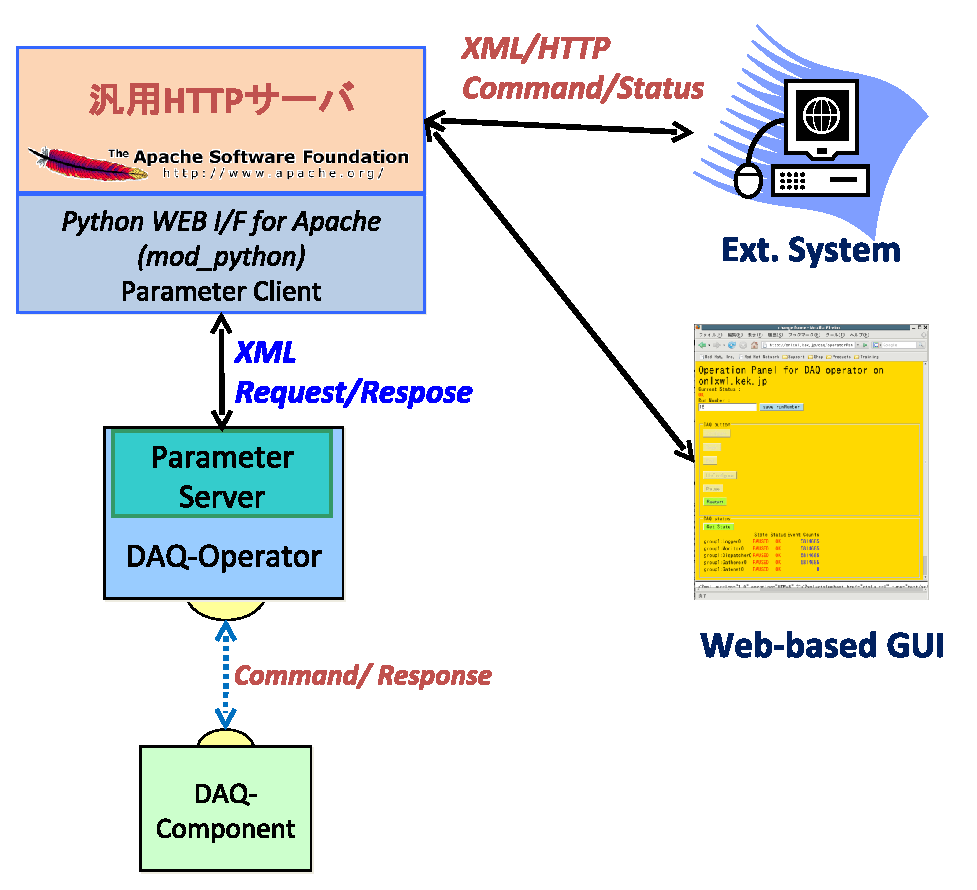
\includegraphics[width=80mm]{web-interface.eps}
%%   \end{center}
%%   %\vspace{-2mm}
%%   \caption{システム・インターフェイスの概念図}
%%   \label{web-interface.fig}
%% \end{wrapfigure}



%%この機能を用いたラン・コントロール・パネルやオンライン・ヒストグラムの表示の実装については参考文献 \cite{Web-GUI}を参照してください。

\section{さいごに}
OpenRTM-aist のバージョンアップやDAQミドルウェアの実装の改良により、本解説書で
説明した内容が古くなる可能性があります。また、現状においても説明が十分ではない箇所もありますので、
今後もこの技術解説書の内容を順次更新する予定です。
コメント、ご要望がありましたらお知らせください。

\addcontentsline{toc}{section}{References}
\begin{thebibliography}{99}

 \bibitem{RTM}  産業技術総合研究所 知能システム研究部門 OpenRTM-aistの公式Webサイトを参照。\\
   \url{http://www.openrtm.org/OpenRTM-aist/}
 \bibitem{RTM-OMG} Robotic Technology Component (RTC),Version 1.0\\
   http://www.omg.org/spec/RTC/1.0/
 \bibitem{CHEP06} Y. Yasu, et al., Feasibility of data acquisition middleware based on robot technology, CHEP06, 2006.\\
   \url{http://daqmw.kek.jp/docs/chep06-ID192-paper.pdf}
 \bibitem{OVERVIEW} 仲吉一男、安 芳次、千代浩司、「DAQミドルウェア概要」、2008年11月\\
   \url{http://daqmw.kek.jp/docs/daqmw-overview.pdf}
 \bibitem{RTM-book} 長瀬雅之、中本啓之、池添明宏、「はじめてのコンポーネント指向ロボットアプリケーション開発」、毎日コミュニケーションズ、2008年、ISBN978-4-8399-2900-8.
\bibitem{Cond-manual} 安 芳次、「Conditionデータベースの開発マニュアル」、2009年7月\\
\url{http://daqmw.kek.jp/docs/ConditionDevManual.pdf}
%%\bibitem{Config-manual} 仲吉一男、「DAQミドルウェアのシステム・コンフィグレーション」、2009年7月\\
%%\url{http://greentea.kek.jp/daqm/docs/configuration.pdf}
%%\bibitem{Web-GUI} 安 芳次、「WEBを用いたDAQミドルウェアGUI開発マニュアル」、2009年7月\\
\url{http://greentea.kek.jp/daqm/docs/WebDAQGUI.pdf}
\end{thebibliography}


\newpage
\appendix
\section{XML/HTTPプロトコル}\label{xmlhttp}
DAQミドルウェアと外部システムとの通信に使用するXML/HTTPプロトコルを表\ref{http1.tab}と表\ref{http2.tab}に示します。
\begin{table}[htbp]
\begin{center}
{\scriptsize
    \begin{tabular}{|c|c|c|l|l|}\hline
      コマンド    & 要求/応答 & メソッド & URI                      & HTTP ボディ\\ \hline
                  & 要求      & POST & http://xxx/daq/operatorPanel/run.py/Params & \verb|cmd="<?xml version="1.0" encoding="UTF-8" ?>|\\
                  &           &      &                                            & \verb|<request>|\\ 
                  &           &      &                                            & \verb|  <params>config.xml</params>|\\
                  &           &      &                                            & \verb|</request>"|\\ \cline{2-5}
                  &           &      &                                            & \verb|<?xml version="1.0" encoding="UTF-8" ?>|\\ 
                  &           &      &                                            & \verb|<response>|\\ 
                  &           &      &                                            & \verb|  <methodName>Params</methodName>|\\ 
                  &           &      &                                            & \verb|  <returnValue>|\\ 
                  &           &      &                                            & \verb|    <result>|\\ 
      CONFIGURE   & 応答      &      &                                            & \verb|      <status>OK</status>|\\ 
                  &           &      &                                            & \verb|      <code>0</code>|\\ 
                  &           &      &                                            & \verb|      <className/>|\\ 
                  &           &      &                                            & \verb|      <name/>|\\ 
                  &           &      &                                            & \verb|      <methodName/>|\\ 
                  &           &      &                                            & \verb|      <messageEng/>|\\ 
                  &           &      &                                            & \verb|      <messageJpn/>|\\ 
                  &           &      &                                            & \verb|    <result>|\\ 
                  &           &      &                                            & \verb|  </returnValue>|\\ 
                  &           &      &                                            & \verb|  </returnValue>|\\ 
                  &           &      &                                            & \verb|</response>|\\ \hline

                  & 要求      & POST & http://xxx/daq/operatorPanel/run.py/Begin  & \verb|cmd="<?xml version="1.0" encoding="UTF-8" ?>|\\
                  &           &      &                                            & \verb|<request>|\\ 
                  &           &      &                                            & \verb|  <runNo>1</runNo>|\\
                  &           &      &                                            & \verb|</request>"|\\ \cline{2-5}
                  &           &      &                                            & \verb|<?xml version="1.0" encoding="UTF-8" ?>|\\ 
                  &           &      &                                            & \verb|<response>|\\ 
                  &           &      &                                            & \verb|  <methodName>Begin</methodName>|\\ 
                  &           &      &                                            & \verb|  <returnValue>|\\ 
                  &           &      &                                            & \verb|    <result>|\\ 
      START       & 応答      &      &                                            & \verb|      <status>OK</status>|\\ 
                  &           &      &                                            & \verb|      <code>0</code>|\\ 
                  &           &      &                                            & \verb|      <className/>|\\ 
                  &           &      &                                            & \verb|      <name/>|\\ 
                  &           &      &                                            & \verb|      <methodName/>|\\ 
                  &           &      &                                            & \verb|      <messageEng/>|\\ 
                  &           &      &                                            & \verb|      <messageJpn/>|\\ 
                  &           &      &                                            & \verb|    <result>|\\
                  &           &      &                                            & \verb|  </returnValue>|\\ 
                  &           &      &                                            & \verb|</response>|\\ \hline

                  & 要求      & POST & http://xxx/daq/operatorPanel/run.py/End    & \\ \cline{2-5}
                  &           &      &                                            & \verb|<?xml version="1.0" encoding="UTF-8" ?>|\\
                  &           &      &                                            & \verb|<response>|\\ 
                  &           &      &                                            & \verb|  <methodName>End</methodName>|\\ 
                  &           &      &                                            & \verb|  <returnValue>|\\ 
                  &           &      &                                            & \verb|    <result>|\\ 
                  &           &      &                                            & \verb|      <status>OK</status>|\\ 
      STOP        & 応答      &      &                                            & \verb|      <code>0</code>|\\ 
                  &           &      &                                            & \verb|      <className/>|\\ 
                  &           &      &                                            & \verb|      <name/>|\\ 
                  &           &      &                                            & \verb|      <methodName/>|\\ 
                  &           &      &                                            & \verb|      <messageEng/>|\\ 
                  &           &      &                                            & \verb|      <messageJpn/>|\\ 
                  &           &      &                                            & \verb|    <result>|\\
                  &           &      &                                            & \verb|  </returnValue>|\\ 
                  &           &      &                                            & \verb|</response>|\\ \hline
                  & 要求      & POST & http://xxx/daq/operatorPanel/run.py/ResetPar & \\ \cline{2-5}
                  &           &      &                                            & \verb|<?xml version="1.0" encoding="UTF-8" ?>|\\
                  &           &      &                                            & \verb|<response>|\\ 
                  &           &      &                                            & \verb|  <methodName>ResetParams</methodName>|\\ 
                  &           &      &                                            & \verb|  <returnValue>|\\ 
                  &           &      &                                            & \verb|    <result>|\\ 
                  &           &      &                                            & \verb|      <status>OK</status>|\\ 
    UNCONFIGURE   & 応答      &      &                                            & \verb|      <code>0</code>|\\ 
                  &           &      &                                            & \verb|      <className/>|\\ 
                  &           &      &                                            & \verb|      <name/>|\\ 
                  &           &      &                                            & \verb|      <methodName/>|\\ 
                  &           &      &                                            & \verb|      <messageEng/>|\\ 
                  &           &      &                                            & \verb|      <messageJpn/>|\\ 
                  &           &      &                                            & \verb|    <result>|\\
                  &           &      &                                            & \verb|  </returnValue>|\\ 
                  &           &      &                                            & \verb|</response>|\\ \hline
    \end{tabular}
    \caption{外部システムとの通信に使用するXML/HTTP(1)}\label{http1.tab}
}
\end{center}
\end{table}

\begin{table}[htbp]
\begin{center}
{\scriptsize
    \begin{tabular}{|l|c|c|l|l|}\hline
      コマンド    & 要求/応答 & メソッド & URI                      & HTTP ボディ\\ \hline
                  & 要求      & POST & http://xxx/daq/operatorPanel/run.py/Pause  & \\ \cline{2-5}
                  &           &      &                                            & \verb|<?xml version="1.0" encoding="UTF-8" ?>|\\
                  &           &      &                                            & \verb|<response>|\\ 
                  &           &      &                                            & \verb|  <methodName>Pause</methodName>|\\ 
                  &           &      &                                            & \verb|  <returnValue>|\\ 
                  &           &      &                                            & \verb|    <result>|\\ 
                  &           &      &                                            & \verb|      <status>OK</status>|\\ 
    PAUSE         & 応答      &      &                                            & \verb|      <code>0</code>|\\ 
                  &           &      &                                            & \verb|      <className/>|\\ 
                  &           &      &                                            & \verb|      <name/>|\\ 
                  &           &      &                                            & \verb|      <methodName/>|\\ 
                  &           &      &                                            & \verb|      <messageEng/>|\\ 
                  &           &      &                                            & \verb|      <messageJpn/>|\\ 
                  &           &      &                                            & \verb|    <result>|\\
                  &           &      &                                            & \verb|  </returnValue>|\\ 
                  &           &      &                                            & \verb|</response>|\\ \hline
                  & 要求      & POST & http://xxx/daq/operatorPanel/run.py/Restart & \\ \cline{2-5}
                  &           &      &                                            & \verb|<?xml version="1.0" encoding="UTF-8" ?>|\\
                  &           &      &                                            & \verb|<response>|\\ 
                  &           &      &                                            & \verb|  <methodName>Restart</methodName>|\\ 
                  &           &      &                                            & \verb|  <returnValue>|\\ 
                  &           &      &                                            & \verb|    <result>|\\ 
                  &           &      &                                            & \verb|      <status>OK</status>|\\ 
    RESUME        & 応答      &      &                                            & \verb|      <code>0</code>|\\ 
                  &           &      &                                            & \verb|      <className/>|\\ 
                  &           &      &                                            & \verb|      <name/>|\\ 
                  &           &      &                                            & \verb|      <methodName/>|\\ 
                  &           &      &                                            & \verb|      <messageEng/>|\\ 
                  &           &      &                                            & \verb|      <messageJpn/>|\\ 
                  &           &      &                                            & \verb|    <result>|\\
                  &           &      &                                            & \verb|  </returnValue>|\\ 
                  &           &      &                                            & \verb|</response>|\\ \hline
                  & 要求      & GET  & http://xxx/daq/operatorPanel/run.py/Log    & \\ \cline{2-5}
                  &           &      &                                            & \verb|<?xml version="1.0" encoding="UTF-8" ?>|\\
                  &           &      &                                            & \verb|<response>|\\ 
                  &           &      &                                            & \verb|  <methodName>Restart</methodName>|\\ 
                  &           &      &                                            & \verb|  <returnValue>|\\ 
                  &           &      &                                            & \verb|    <result>|\\ 
                  &           &      &                                            & \verb|      <status>OK</status>|\\ 
                  &           &      &                                            & \verb|      <code>0</code>|\\ 
                  &           &      &                                            & \verb|      <className/>|\\ 
                  &           &      &                                            & \verb|      <name/>|\\ 
                  &           &      &                                            & \verb|      <methodName/>|\\ 
                  &           &      &                                            & \verb|      <messageEng/>|\\ 
                  &           &      &                                            & \verb|      <messageJpn/>|\\ 
    GET LOG       & 応答      &      &                                            & \verb|    <result>|\\
                  &           &      &                                            & \verb|    <logs>|\\
                  &           &      &                                            & \verb|      <log>|\\
                  &           &      &                                            & \verb|        <compName>READER</compName>|\\
                  &           &      &                                            & \verb|        <state>RUNNING</state>|\\
                  &           &      &                                            & \verb|        <eventNum>100</eventNum>|\\
                  &           &      &                                            & \verb|        <compStatus>WORKING</compStatus>|\\
                  &           &      &                                            & \verb|      </log>|\\
                  &           &      &                                            & \verb|      <log>|\\
                  &           &      &                                            & \verb|        <compName>MONITOR</compName>|\\
                  &           &      &                                            & \verb|        <state>RUNNING</state>|\\
                  &           &      &                                            & \verb|        <eventNum>100</eventNum>|\\
                  &           &      &                                            & \verb|        <compStatus>WORKING</compStatus>|\\
                  &           &      &                                            & \verb|      </log>|\\
                  &           &      &                                            & \verb|    </logs>|\\
                  &           &      &                                            & \verb|  </returnValue>|\\ 
                  &           &      &                                            & \verb|</response>|\\ \hline

    \end{tabular}
    \caption{外部システムとの通信に使用するXML/HTTP(2)}\label{http2.tab}

}
\end{center}
\end{table}

\newpage
\section{DAQコンポーネントの実装に使用する関数一覧}\label{funclist}

\newcommand{\myfunc}[3]{
\vspace{2mm}
    \begin{tabular}{ c l }
      名前 &             \\
           & \texttt{#1} \\
      書式 &             \\
           & \small{\texttt{#2}}\\
      説明 &             \\
           & p.\texttt{#3} \\
    \end{tabular}
\begin{center}
\begin{minipage}{15cm}
\hrule width 15cm
\end{minipage}
\end{center}
}

\myfunc{init\_command\_port - コマンドポート初期化}{int init\_command\_port()}{\pageref{init} \ref{init}}
\myfunc{init\_state\_table() - 状態遷移テーブルの初期化}{void init\_state\_table()}{\pageref{init} \ref{init}}
\myfunc{set\_comp\_name(char{*} name) - コンポーネント名設定}{int set\_comp\_name(char{*} name)}{\pageref{init} \ref{init}}
\myfunc{inc\_sequence\_num() }{int inc\_sequence\_num() }{\pageref{seq} \ref{seq}}
\myfunc{reset\_sequence\_num() }{int reset\_sequence\_num() }{\pageref{seq} \ref{seq}}
\myfunc{get\_sequence\_num() }{unsigned long long get\_sequence\_num() }{\pageref{seq} \ref{seq}}
\myfunc{inc\_total\_data\_size }{int inc\_total\_data\_size(unsigned int byteSize)}{\pageref{datasize} \ref{datasize}}
\myfunc{reset\_total\_data\_size }{int reset\_total\_data\_size() }{\pageref{datasize} \ref{datasize}}
\myfunc{get\_total\_data\_size }{unsigned long long get\_total\_data\_size() }{\pageref{datasize} \ref{datasize}}
\myfunc{set\_header }{int set\_header(unsigned char{*} header, unsigned int data\_byte\_size) }{\pageref{header} \ref{header}}
\myfunc{set\_footer }{set\_footer(unsigned char{*} footer, unsigned int sequence\_num) }{\pageref{header} \ref{header}}
\myfunc{check\_header }{bool check\_header(unsigned char{*} header, unsigned int received\_byte) }{\pageref{header} \ref{header}}
\myfunc{check\_footer }{bool check\_footer(unsigned char{*} footer, unsigned int loop\_cnt) }{\pageref{header} \ref{header}}
\myfunc{check\_header\_footer }{bool check\_header\_footer(const RTC::TimedOctetSeq\& in\_data,unsigned int block\_byte\_size)}{\pageref{header} \ref{header}}
\myfunc{get\_event\_size }{unsigned int get\_event\_size(unsigned int block\_byte\_size) }{\pageref{header} \ref{header}}
\myfunc{check\_trans\_lock}{bool check\_trans\_lock() }{\pageref{state} \ref{state}}
\myfunc{set\_trans\_unlock}{bool set\_trans\_unlock() }{\pageref{state} \ref{state}}
\myfunc{fatal\_error\_report}{void fatal\_error\_report(FatalType::Enum type, int code = -1) }{\pageref{fatal} \ref{fatal}}
\myfunc{fatal\_error\_report}{void fatal\_error\_report(FatalType::Enum type, const char* desc,int code = -1) }{\pageref{fatal} \ref{fatal}}
\myfunc{check\_outPort\_status}{BufferStatus check\_outPort\_status(RTC::OutPort<RTC::TimedOctetSeq> \& outPort) }{\pageref{portstat} \ref{portstat}}
\myfunc{check\_inPort\_status}{BufferStatus check\_inPort\_status(RTC::InPort<RTC::TimedOctetSeq> \& inPort) }{\pageref{portstat} \ref{portstat}}

\newpage
\section{config.xsd}\label{config.xsd}
コンフィグレーションファイルのXMLスキーマを下記に示します。
\VerbatimInput{config.xsd}

\end{document}
